% Allow relative paths in included subfiles that are compiled separately
% See https://tex.stackexchange.com/questions/153312/

\providecommand{\main}{..}
\newcommand{\decfirst}{\textit{Decision.1}}
\newcommand{\decsecond}{\textit{Decision.2}}
\documentclass[\main/thesis.tex]{subfiles}

\externaldocument{}


\begin{document}

\chapter{The Virtual Ear}
\section{Why Do We Need A Virtual Ear?}
\label{sec:ear}
In the previous chapters, we conceptualized a system that can generate new drum sounds using a virtual source of random sounds, and an automatic ear that can pick out sounds which resemble drums. The virtual synthesizer was introduced in the previous chapter. What is needed now is a tool which can automatically separate the sounds which resemble percussion from those which do not. Here, what we refer to as an \enquote{ear} is any method of scoring and classifying audio (e.g machine listening) \cite{malkin2006machine,rowe1992interactive}. The ideal virtual ear will be capable of receiving a piece of audio and scoring it based on how well it satisfies certain criteria. In the scope of this project, the virtual ear must receive the random sounds generated by the virtual synthesizer, and separate those resembling drums from non-drums, and categorize the type of drums. 
 
\section{Implementation Steps}
To create a virtual ear, we use machine learning algorithms. In order for these algorithms to work as intended, they must be given examples of drum and non-drum data. Here, the datasets of drum and non-drum sounds discussed in Chapter~\ref{sec:datasets} are utilized. In order to speed up training times, we do not train our models on raw audio data, rather, we define two different transformation functions which project audio data into smaller spaces. These transformation functions can also be thought of as feature extraction steps. These functions are discussed in Section~\ref{chap:represent_sound}. In Section~\ref{sec:decisions}, the implementation and measurements of two different model types are discussed.

% The high-level approach to training is depicted in figure~\ref{fig:ear_plan}.
\subsection{Learning Caveats}
To train the models, percussive sounds are used as positive examples, while synthesizer sounds are used as negatives. Figure~\ref{fig:ven_data} highlights critical problems with the learning approach. The change in learning domains---particularly with the case of positive examples of percussive instruments---should not interfere with transformation of knowledge from the training of the ear to the hearing test. 

\begin{figure}[]
    \begin{center}
    \textbf{Data Overview}
    \makebox[\textwidth]{
    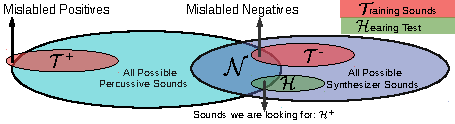
\includegraphics[width=1\linewidth]{images/chapter_4/venn_data.pdf}}
    \end{center}
    \caption{ An illustration of the discrepancy between the sounds used to train the classifiers and the type of sounds the classifier is expected to classify. $\mathcal{N}$ is the set of percussive sounds a synthesizer is capable of making. The inclusion of sounds in this group may vary from person to person. The positive samples, $\mathcal{T^{+}}$, is a small fraction of a wide variety of percussive sounds that are conceivable. For $\mathcal{T^{-}}$, Any number of random samples can be generated. $\mathcal{H}$ is a series of sounds sent to the ear for classification.}
\label{fig:ven_data}
\end{figure}

Traditional classification tasks often make the assumption the data points used for training the model and future unlabeled data will emerge from the same system of processes~\cite{geng2020recent,mundt2019open}. This assumptions requires that sufficient positive examples of all possible classes exist and are trained on. Works which involve the implementation of GANs have documented scenarios in which networks will assign high categorization probabilities to nonsensical, out of context data which should be rejected rather than categorized~\cite{geng2020recent,mundt2019open,hassen2020learning}. This issue is reflective of the open set recognition (OSR) problem~\cite{geng2020recent,mundt2019open}, where learning by examples can prove difficult when the category that is being learned is infinitely large. 

We consider drum sounds to be a closed set, since it is reasonable that a sufficiently large sample pack can effectively describe common drum categories, while effective representation of all possible non-drum sounds is not attainable via examples alone. A hurdle towards the implementation of a \enquote{drum from non-drum} recognizer is that the set of sounds that are not drums do not share any characteristics beyond~\enquote{not being a drum}, making the learning process using negative examples difficult.  To ensure the quality of the results, particularly in the categorization of drums from non-drums, manual hearing tests need to be conducted to measure the quality of the results. The results of our blinded hearing tests are discussed in Chapter~\ref{surveys}.

\section{Representing Sound}
\label{chap:represent_sound}
We are looking to implement machine learning models capable of analyzing sounds. Machine learning algorithms learn from observing data, which in the scope of this project is audio signals. Therefore, it is important to establish how digital sound will be transformed before an algorithm attempts to learn from it. 

Raw digital sound can be difficult to analyze as a single second of digital sound at our desired sample rate exists as an array of 48000 numbers. The choice of feature extraction from digital sound is a foundational step towards the implementation of the virtual ear. While smaller representations can reduce computation costs significantly, important features may be lost in the transformation. Put differently, we wish to transform sounds into a small feature space without the loss of critical information. We take two approaches towards this goal: \begin{enumerate}
    \item By using features extracted from Fourier Transformations of sounds \item By using features extracted from autoencoders which condense the Fourier transformations. 
\end{enumerate}
\subsection{Fourier Transforms}
\label{sec:fourier_transforms}
In this work we rely on derivatives of the fast Fourier transform (FFT), and by extension, short-time Fourier transforms (STFT) for feature extraction. Various works have demonstrated effective reconstruction of signals given their short-time Fourier transforms~\cite{nawab1983signal,griffin1984signal}. If the STFT of a signal can be used for its reconstruction, perhaps it can be utilized as a source of fundamental features~\cite{lee2009unsupervised,huzaifah2017comparison}. Using FFT, a signal can be represented by a vector with each index corresponding to a frequency-bin (a range of frequencies too close to be distinguishable) and the value at each index corresponding to the combined-magnitude of the frequencies within the bin. STFT can be employed when temporal changes in frequency bins are of interest; this can be done by the application of FFT\footnote{more accurately, discrete Fourier transforms} to a sliding time-window on the signal to create a vector for each time step. This matrix can effectively represent the frequencies present in the signal at each time step, given the right window-length and hop-size (how much the window is shifted at each time-step). 

To extract the FFT feature sets from a signal, we defined the following 3 transformation functions. These functions are applied at training time to transform raw digital signals into simpler formats, which may be easier to learn from: 
\begin{figure}
\centering
\textbf{Visual Representation of Raw Features}\par\medskip
    \subcaptionbox{Recorded hat sample}{    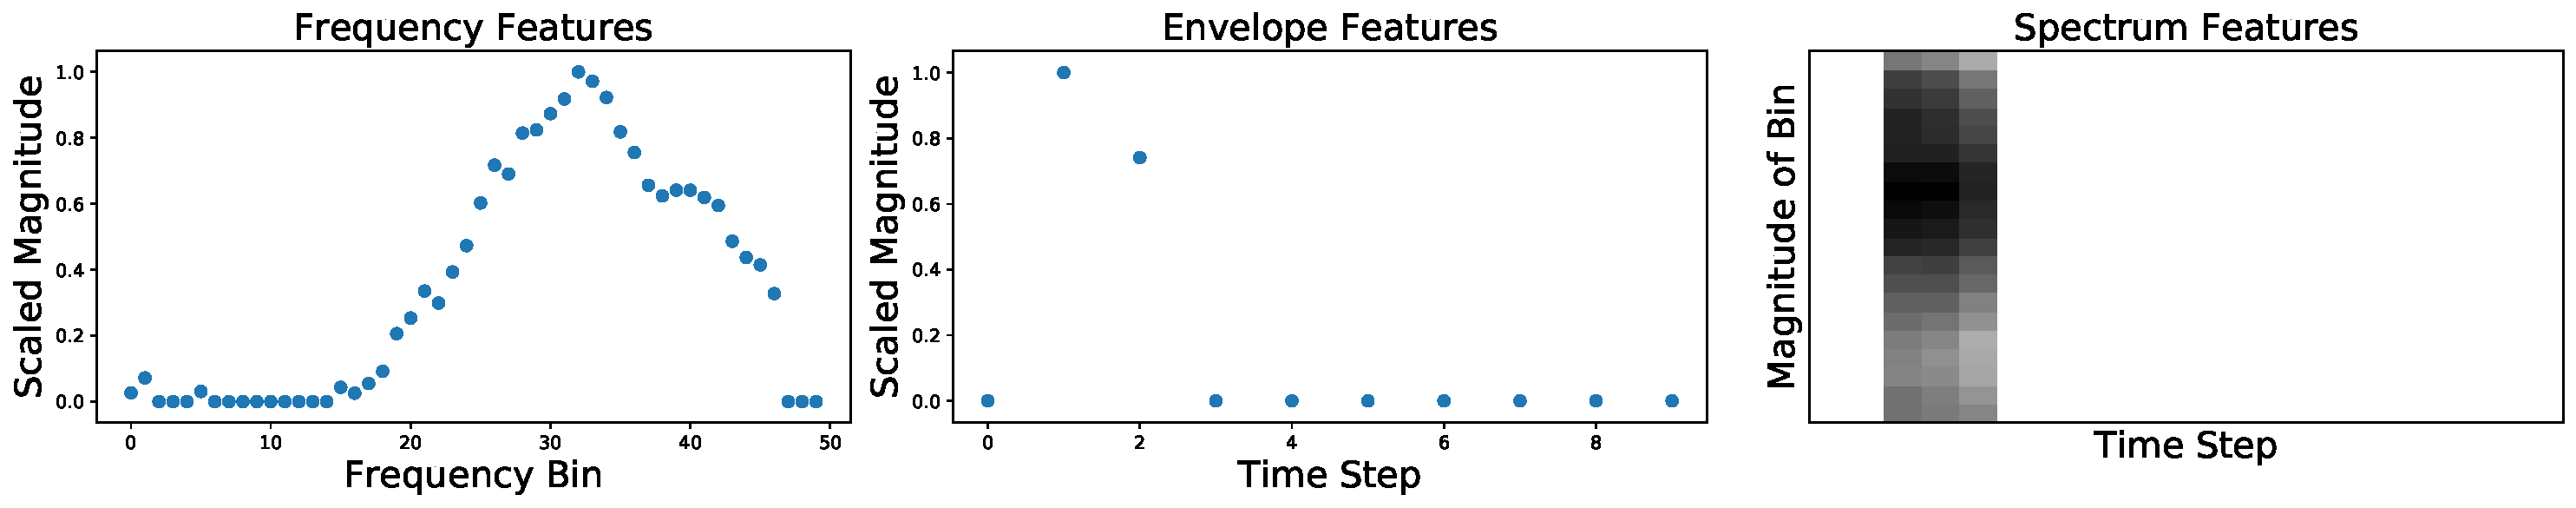
\includegraphics[width=1\columnwidth]{images/ff1.pdf}
    }
    \subcaptionbox{Randomly generated audio with percussive qualities, resembling a tight snare}{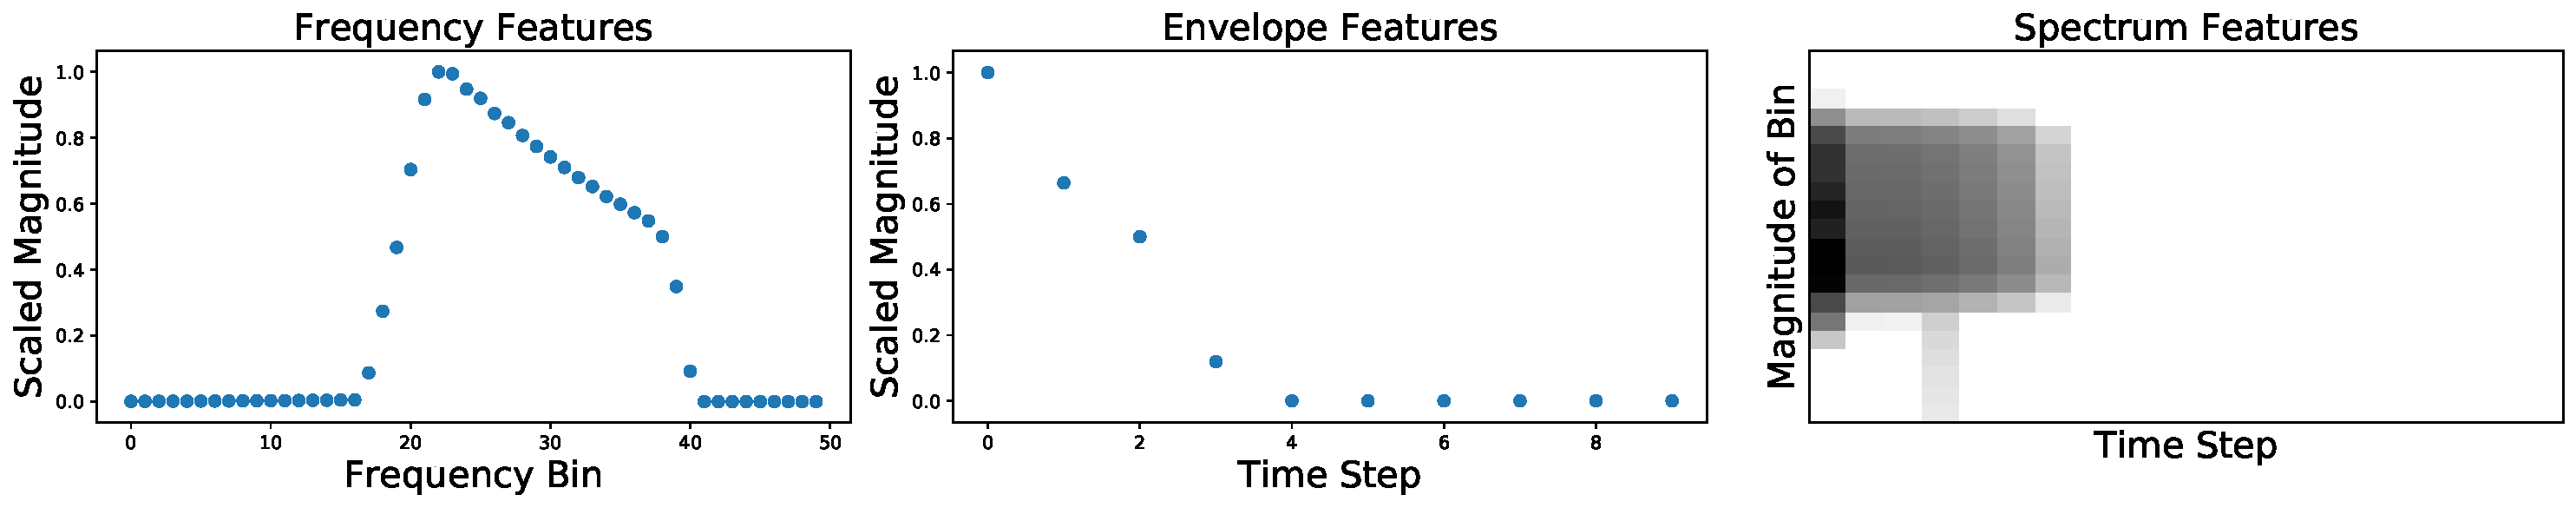
\includegraphics[width=1\columnwidth]{images/ff2.pdf}}
    \subcaptionbox{A randomly generated noise with a percussive envelop but non-percussive frequency features (modulated pitch)}
    { 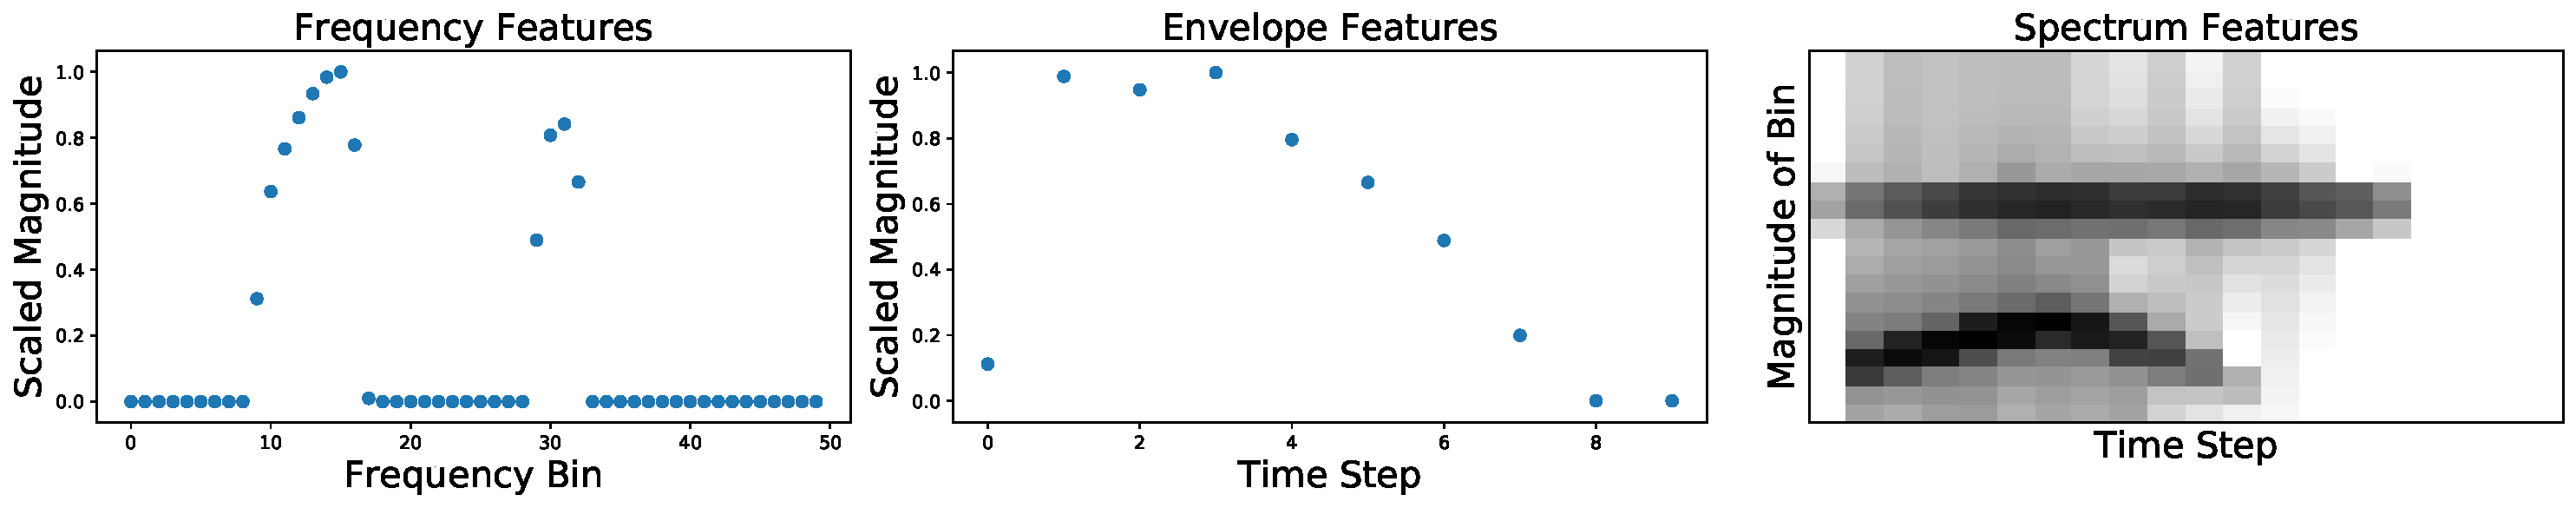
\includegraphics[width=1\columnwidth]{images/ff3.pdf}}
\caption{Graphed representation of features extracted for 3 different samples. Sample $a$ is a recorded hat from our database. sample $b$ is an example of randomly generated noise with percussive qualities that we found suitably similar to a snare sound. Sample $c$ is an example of a randomly generated noise where the spectrum features are necessary for proper classification.}
\label{fig:stackspectrums}
\end{figure}
\begin{enumerate}
\item Envelope Transformation: The goal of this feature is to capture the changes in loudness for the duration of the signal. Using STFT we generate a matrix $M_{i \times j}$ with rows $i$ and columns $j$ corresponding to time steps and frequency bins respectively, and with values $v_{i \times j}$ indicating the magnitude of the frequency bin $j$ at each time-step $i$. Information about the envelope of the signal can be extracted by summing the values of $M$ for each time-step (or row $i$), giving us a feature vector $v_i$. This vector is then normalized to the range of 0 to 1. The information contained in this vector is similar to that of an RMS measurement.
\item Frequency Transformation: A static, normalized snap-shot of the  frequencies present within the audio. The calculation of this feature vector is similar to the envelope, but the summation is done along the frequency axis.
\item Spectrum Transformation: STFT with its values normalized from 0-1. Since this feature is a 2D matrix rather than a vector, it captures more information about our signal. This spectrogram is \enquote{mel-scaled}\cite{stevens1940relation} to better represent human perception of audio frequencies.
\end{enumerate}

Once the transformation functions are applied to a signal, we have 3 feature sets which can be learned from. The Frequency bin and envelope features are 1 dimensional arrays of values in the 0-1 range, and are given directly to the learning models. The spectrum features are a 2 dimensional array of values in the 0-1 range, which can be thought of as a greyscale image. Depending on the the learning algorithm, the spectrum features may be flattened into a single dimension (e.g fully connected neural net) or left unchanged (e.g convolutional neural net). 

We now have 3 types of which can be used for learning. Next, in Section~\ref{section:embedded_feats}, we discuss how the spectrum features can be further encoded, or condensed, using autoencoder neural networks. The procedure of learning from these feature sets is covered in Section~\ref{sec:decisions}. Section~\ref{TPE_models} discusses the training procedure for models which directly use the FFT features described above, and models which use encoded spectrum features are discussed in Section~\ref{chap3:mixed_ear_models}.

\subsection{Embedded FFT Features}
\label{section:embedded_feats}
\begin{figure}[t!]
    \begin{center}
    \textbf{AutoEncoding Spectrograms}
    \makebox[\textwidth]{
    \fbox{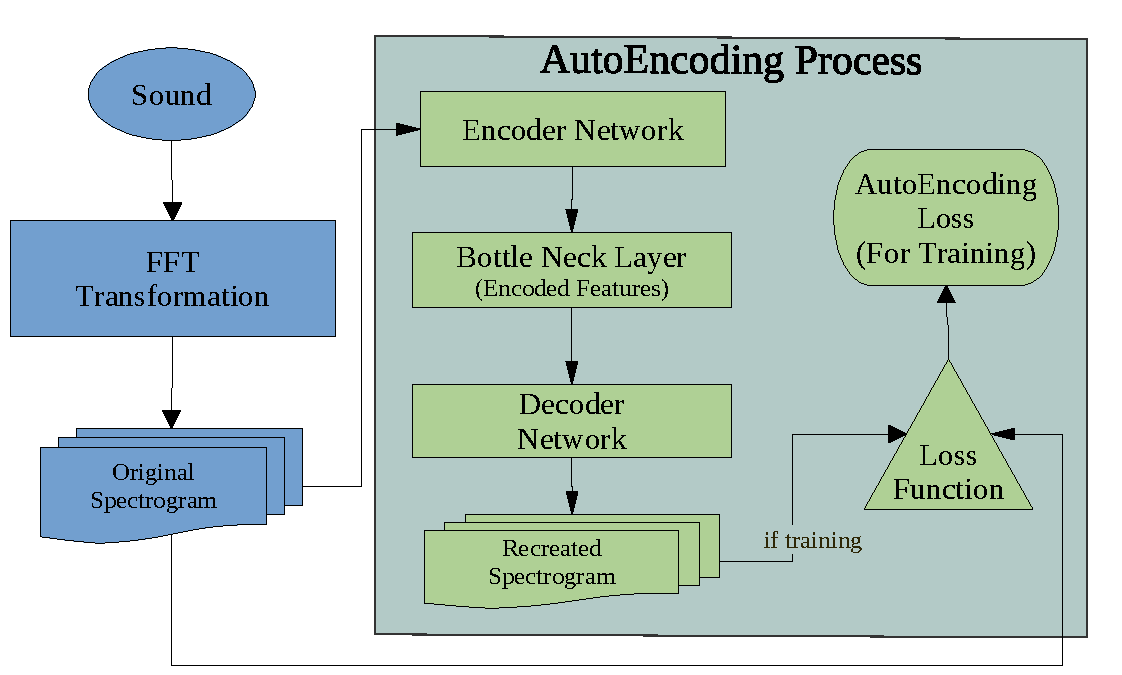
\includegraphics[width=1.1\linewidth]{images/autoencoder.pdf}}}
    \end{center}
    \caption{Overview of autoencoder training. Once an autoencoder is trained, the decoder and loss function are not needed, and the bottleneck layer values will be used as features. }
\label{fig:autoencoder}
\end{figure}

% http://www.justinsalamon.com/uploads/4/3/9/4/4394963/cramer_looklistenlearnmore_icassp_2019.pdf says they need almost 40 million samples 
% http://www.cs.toronto.edu/~zemel/documents/prototypical_networks_nips_2017.pdf
% 
The advantage of the spectrum features discussed earlier is that it contains temporal information for the amplitude of each frequency bin. This means that it contains both envelope and frequency features, along with other possibly useful information. This comes at the cost of being exponentially larger than either frequency or envelope features. To speed up and simplify training, we want to further reduce the dimensionality of the spectrum features, ideally without the loss of vital information needed for classification. For this purpose, we utilized autoencoder networks, which are an approach to dimensionality reduction using deep neural networks~\cite{hinton1994autoencoders,hinton2006reducing}. 

Autoencoders are comprised of an encoder and a decoder. The encoder has the task of meaningfully projecting the spectrum data of each sound onto a small bottleneck layer, while the decoder aims to use this projection to replicate the input data as closely as possible. Successful training will lead to an encoder network capable of projecting audio data into a low dimensional vector. Here, the original data is the spectrum features, and the encoding at the bottle neck layer is the simplified feature sets which we would like to use for training. With some luck, this low dimensional vector will contain vital information which can be used for training models much faster than using the original data, with little loss in performance. The autoencoder training process is depicted in Figure~\ref{fig:autoencoder}.
\begin{table}[h!]

\begin{tabular}{|p{28mm}|p{50mm}|p{21mm}|p{21mm}|}
\hline
Hyper-Param. & Description  & Values & Distribution\\ \hline
Model Type      &   Affects encoder's first hidden layer & CNN,FC & Categorical \\  \hline
Optimizer       & Updates network's weights based on loss & Adam,SGD & Categorical  \\  \hline
Hidden Layers   & Extra hidden layer for the Encoder & True,False & Categorical \\  \hline
Time Steps & Temporal granularity of the spectrogram. Affects FFT windowing. & 10,20 & Categorical  \\ \hline
Learning Rate   &    Optimizer's learning rate  & $1^{-4}$ ... $1^{-1}$ & Uniform      \\ \hline
Frequency Bins & Number of spectrogram frequency bins & 10, 30,60 & Categorical \\ \hline

Regularization  &  L2 regularization parameter. Penalizes large weights to prevent overfitting & 1^{-6}~...~1^{-1} & Uniform\\ \hline
Latent Size & Size of bottle neck layer or number encoded features & 8,16,64 & Categorical              \\ \hline
Dropout Rate & Random zeroing of activations between layers to prevent over-fitting & 0,0.5,0.1 & Categorical\\  \hline
\end{tabular}
\caption{The Hyper-Paramter space in which the optimization was conducted.}
\label{table:hyper_params}
\end{table}

\subsection{Architecture and Hyper-Parameter Optimization}
% could do multi-objective pareto front stuff
We make the assumption that if an autoencoder can accurately encode and decode a spectrogram, then the values at the bottleneck layer form a viable alternative to the spectrogram features, while being much smaller in size. Based on this assumption, the optimization goal when training the autoencoder networks is to minimize the difference between the original and decoded spectrogram.  The autoencoder designs used in this project were kept relatively simple, all with approximately 150,000 parameters. Important to mention is that reported loss values of the models do not necessarily reflect whether the encoder will capture data that is useful for any purpose other than being utilized by the decoder. 

These small networks train quickly without the need for much data. Here, we did not give any examples of synthetic noise to the encoders, and only train on organic drums. We hypothesize that if a synthetic noise has drum-like characteristics, its compressed, latent representation given by the encoder will be similar to those of drum sounds and vice versa. In Section~\ref{table:mem_model_selection}, we use these latent expressions to train several machine learning models.

Within the context of machine learning, a model's \emph{hyper-parameters} are fixed parameters which are set before the training begins (e.g., number of layers, size of layers, loss function) and are not learned during the minimization procedure~\cite{bengio2000gradient}. Also within this context, hyper-parameter optimization is the task of searching for a set of hyper-parameters which would maximize the model's capacity, often done by a series of automatic test trials~\cite{bengio2000gradient,bergstra2011algorithms,bergstra2012random}. As a wide variety of viable autoencoder architectures have been proposed~\cite{aouameur2019neural,esling2018generative,gensler2016deep,zhang2016facing,pu2016variational}, we are faced with a number of choices for autoencoder design. To assist with the construction of the model, a number of possible choices for the architecture and the transformation function were defined (see Table~\ref{table:hyper_params}). These choices were then used in hyper-parameter optimization to extract promising sets of values. 

The list of possible choices for the hyper-parameters can be found in Table~\ref{table:hyper_params}. The batchsize $\mathcal{B}$, was set to 64 for training and 4 for testing. We included not only model parameters but also spectrogram transformation parameters within this search space, as GPU accelerated FFT calculations allows ad hoc audio transformations to take place parallel to the training process. We implemented 3 base models which are affected by these hyper-parameters. The \enquote{Model Type} parameter dictates whether CNN or fully connected models are selected. If a \enquote{fully connected} model is selected, the \enquote{hidden layers} parameter selects between the two implementations. The specifications for these models can be found in Tables~\ref{table:FC1_AUTOENCODER},~\ref{table:FC2_AUTOENCODER} and~\ref{table:CNNAUTOENCODER}.

\begin{table}[]
\begin{tabular}{|p{28mm}|p{25mm}|p{23mm}|p{50mm}|}
\hline
Layer-\# & Out Shape & Param Num & Details  \\ \hline
Conv2d-1 & [$\mathcal{B}$, 8, 30, 20] &   208 & Encoder's input \newline
Num. Channels:8\newline
kernel:5x5\newline                  
stride:1\newline    
padding:2 \\ \hline
ReLU-2 & [$\mathcal{B}$, 8, 30, 20] &   0 & \\  \hline
MaxPool2d-3 & [$\mathcal{B}$, 8, 15, 10] & 0 &  kernel:5x5 \newline
stride:2 \\ \hline
Dropout-4 & [$\mathcal{B}$, 8, 15, 10] & 0 &  \\ \hline
Linear-5 & [$\mathcal{B}$, 8] & 9,608 & Encoder's output \\ \hline
Linear-6 & [$\mathcal{B}$, 256] & 2,304 & Decoder's Input \\ \hline
Dropout-7 & [$\mathcal{B}$, 256] & 0 &  \\ \hline
Linear-8 & [$\mathcal{B}$, 600 ] &  154,200& Decoder's output\\ \hline
\end{tabular}
\caption{CNN model design with latent size of 8. 30 and 20 are the assumed frequency bins and step size. Total number of parameters is 166,320. }
\label{table:CNNAUTOENCODER}
\end{table}

\begin{table}[]
\begin{tabular}{|p{28mm}|p{25mm}|p{23mm}|p{50mm}|}
\hline
Layer-\# & Out Shape & Param Num & Details  \\ \hline
Linear-1 & [$\mathcal{B}$, 128]  & 76,928 & Encoder's input \\ \hline
Dropout-2 & [$\mathcal{B}$, 128] & 0 &  \\ \hline
Linear-3 & [$\mathcal{B}$, 8] & 9,608 & Encoder's output \\ \hline
Linear-4 & [$\mathcal{B}$, 128] & 2,304 & Decoder's Input \\ \hline
Dropout-5 & [$\mathcal{B}$, 128]  & 0 &  \\ \hline
Linear-6  & [$\mathcal{B}$, 600 ] &  77,400 &Decoder's output\\ \hline
\end{tabular}
\caption{Fully connected model with only 1 hidden dimension for encoder and decoder. Design assumes latent size of 8. 30 and 20 are the assumed frequency-bins and step-size values. Total number of parameters is 156,512.}
\label{table:FC1_AUTOENCODER}
\end{table}

\begin{table}[]

\begin{tabular}{|p{28mm}|p{25mm}|p{23mm}|p{50mm}|}
\hline
Layer-\# & Out Shape & Param Num & Details  \\ \hline
Linear-1 & [$\mathcal{B}$, 128]  & 76,928 & Encoder's input \\ \hline
Dropout-2 & [$\mathcal{B}$, 128] & 0 &  \\ \hline
Linear-3 & [$\mathcal{B}$, 32]  & 4,128 & \\ \hline
Dropout-4 & [$\mathcal{B}$, 128] & 0 &  \\ \hline
Linear-5 & [$\mathcal{B}$, 8] & 9,608 & Encoder's output \\ \hline
Linear-4 & [$\mathcal{B}$, 32] & 2,304 & Decoder's Input \\ \hline
Dropout-5 & [$\mathcal{B}$, 32]  & 0 &  \\ \hline
Linear-4 & [$\mathcal{B}$, 128] & 2,304 & \\ \hline
Dropout-5 & [$\mathcal{B}$, 128]  & 0 &  \\ \hline
Linear-6  & [$\mathcal{B}$, 600 ] &  77,400 &Decoder's output\\ \hline
\end{tabular}
\caption{Fully connected model with 2 hidden dimensions for encoder and decoder. Design assumes latent size of 8. 30 and 20 are the assumed frequency-bins and step-size values. Total number of parameters is 163,232.}
\label{table:FC2_AUTOENCODER}
\end{table}


Using the optuna optimization tools \cite{akiba2019optuna}, we conducted 500 search trials. The trial's success is measured in their final loss value, calculated by applying the model to test data-set. Here, the test data-set is all sounds from MixedDB. Each trial consisted of 20 epochs of training using a selected set of hyper-parameters. An additional 100 trials with 40 epochs of training were conducted following the initial 500 to test the effect of longer epochs. Each trial's intermediate results (loss at every n epochs where $0<n<20$) were reported to a multi-armed bandit based pruner for early stoppage of unpromising trials\cite{li2017hyperband}. We employed a tree-structured parzen estimator for better navigation of the search space \cite{bergstra2011algorithms,akiba2019optuna} but found short reversions to a random sampling coupled with a decrease in the frequency of pruning helpful in exiting local minima. \\
\begin{figure}[htbp]
\centering
\textbf{Tracing the Best Loss Values}
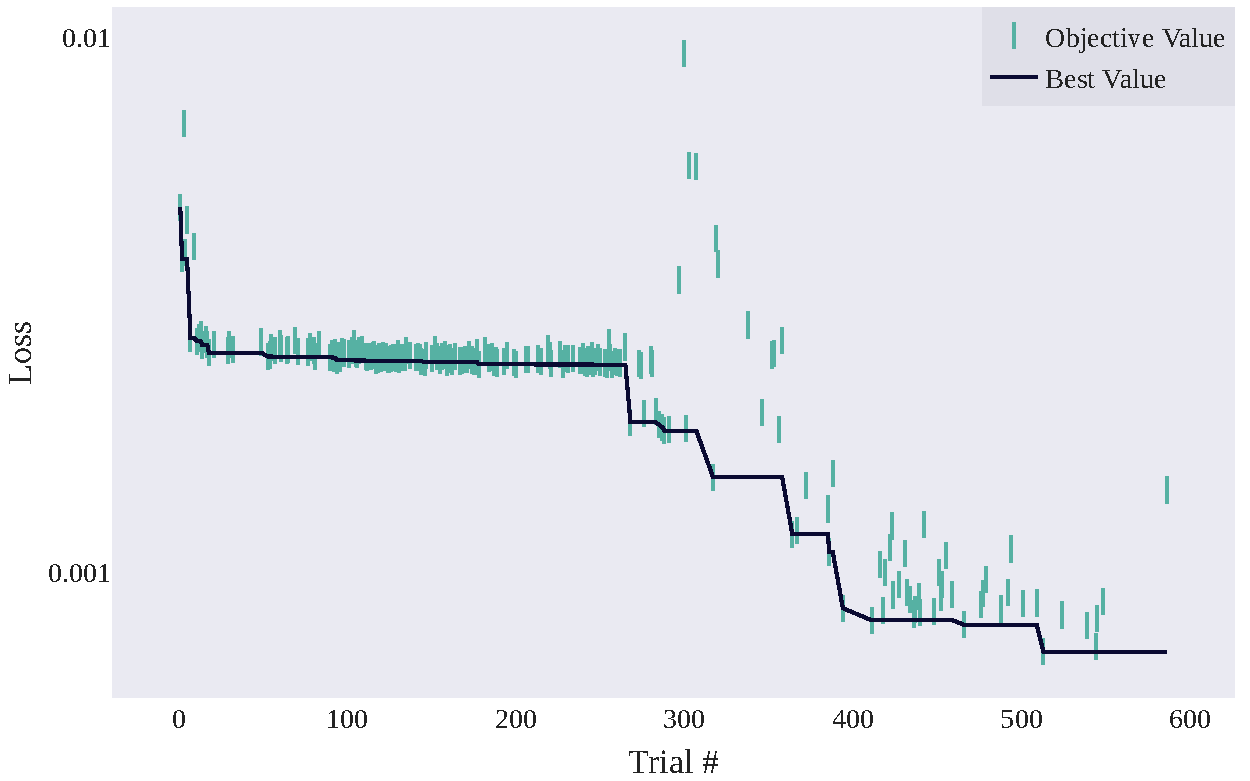
\includegraphics[width=12cm,height=7cm]{images/chapter_3/Optimization_History.pdf}
\caption{Best loss values found during hyper-parameter optimization. The effect of a switch to random sampling and an increase of the pruning threshold can be observed during trials 270 and 310.}
\label{chap3:bestvalues}
\end{figure}

\begin{figure}[]
\centering
\textbf{Loss Value per Epoch for Top 10 Trials}
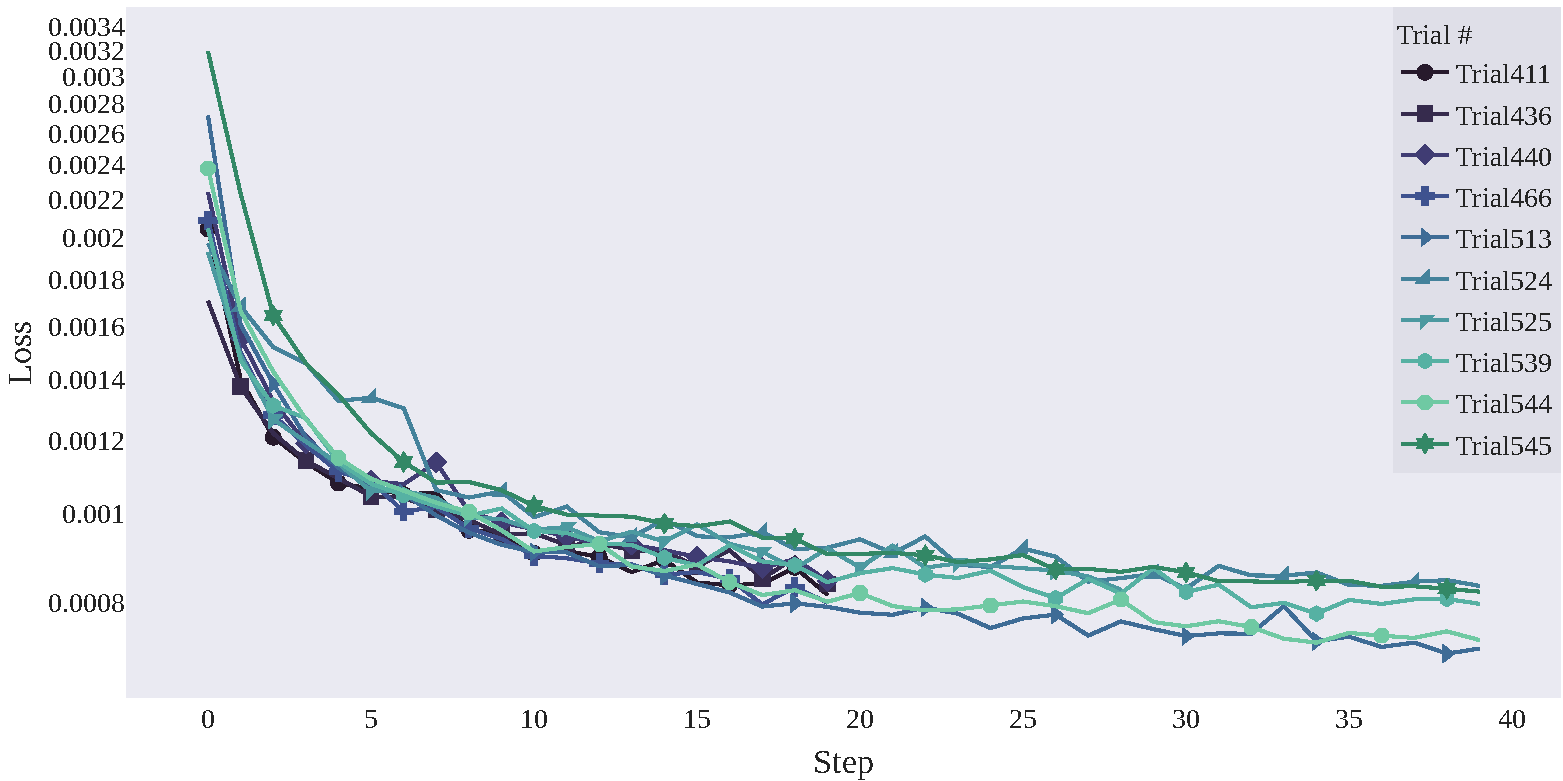
\includegraphics[width=12cm,height=6.5cm]{images/chapter_3/loss_per_training.pdf}
\caption{Loss value per epoch for top 10 trials. Some of the initial 500 trials appear in this list, despite having half the number of epoch steps. The learning curves tend to flatten quickly. Therefore, 20 epoch steps may be a reasonable number for measuring hyper-parameter viability. }
\label{chap3:top10}
\end{figure}


\begin{figure}[]
\begin{center}
    \textbf{Hyper-Parameters' Loss Correlation}
    \makebox[\textwidth]{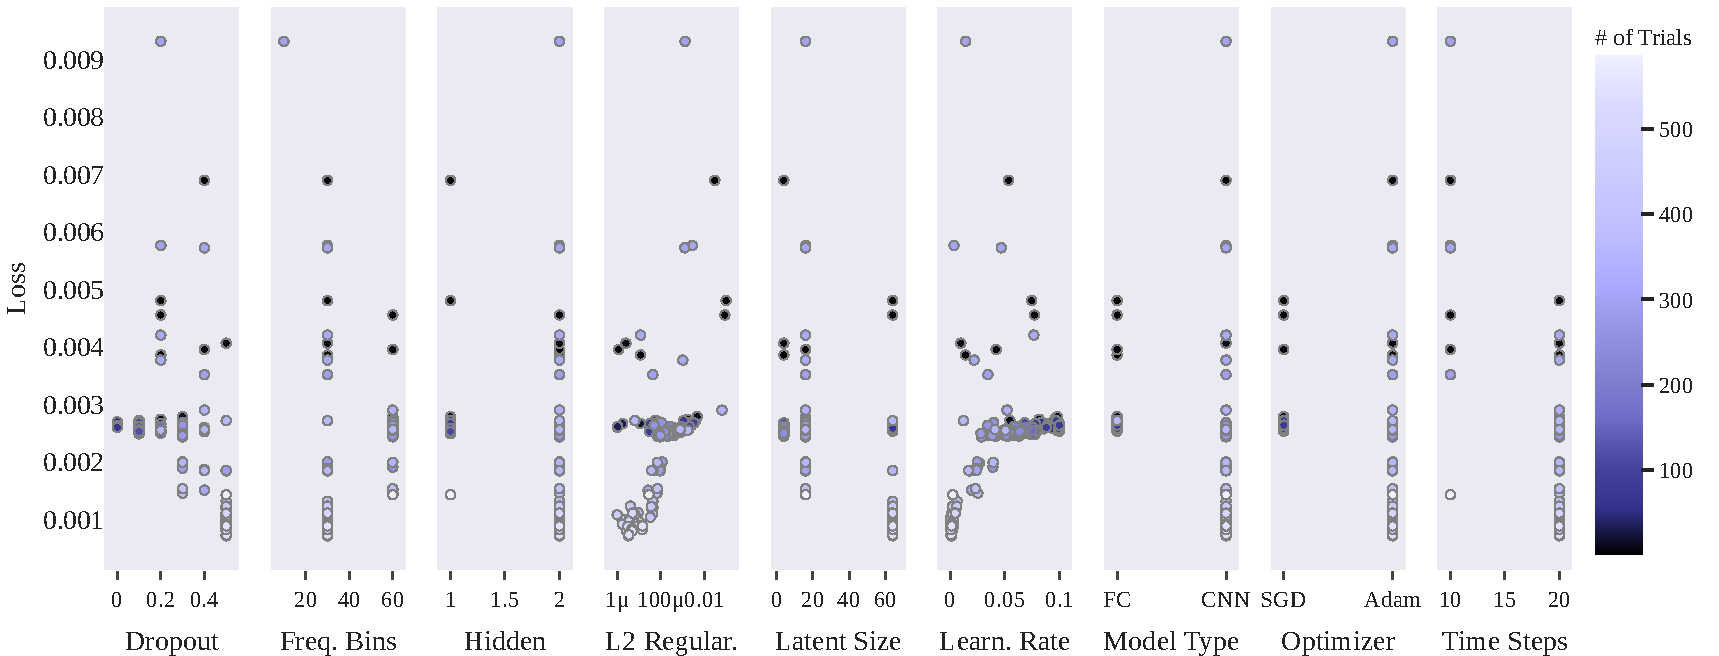
\includegraphics[width=0.95\paperwidth]{images/chapter_3/slice_plot.pdf}}
      \caption{Sliced plot depicting the correlation between hyper-parameters and loss values. The color-scale shows the number of times each parameter has been used in a trial. Our sampling algorithm aims to utilize spaces with higher potential more often. }
    \label{fig:slicegraph}
    \end{center}

\end{figure}
% \begin{figure}[]
% \begin{center}
%     \textbf{ Parallel Coordinates of Hyper-Parameter Sets and Loss}
%     \makebox[\textwidth]{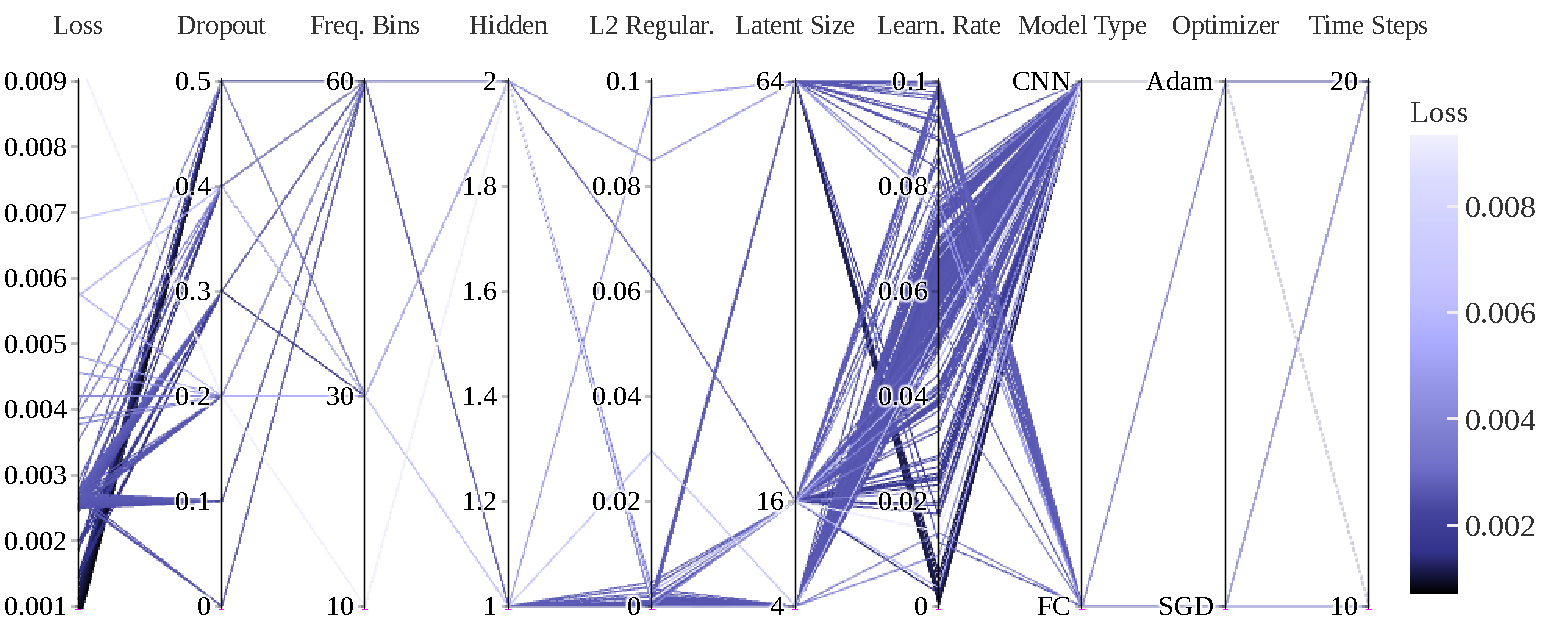
\includegraphics[width=0.9\paperwidth]{images/chapter_3/parallel_coord.pdf}}
%       \caption{Not sure if worth keeping. Paths connect hyper-parameters in a set. Path's are colored based on loss value.}
%       \label{fig:parallel_coord}
%     \end{center}
   
% \end{figure}

\begin{figure}[]
\centering
\textbf{Estimated Parameter Importance}
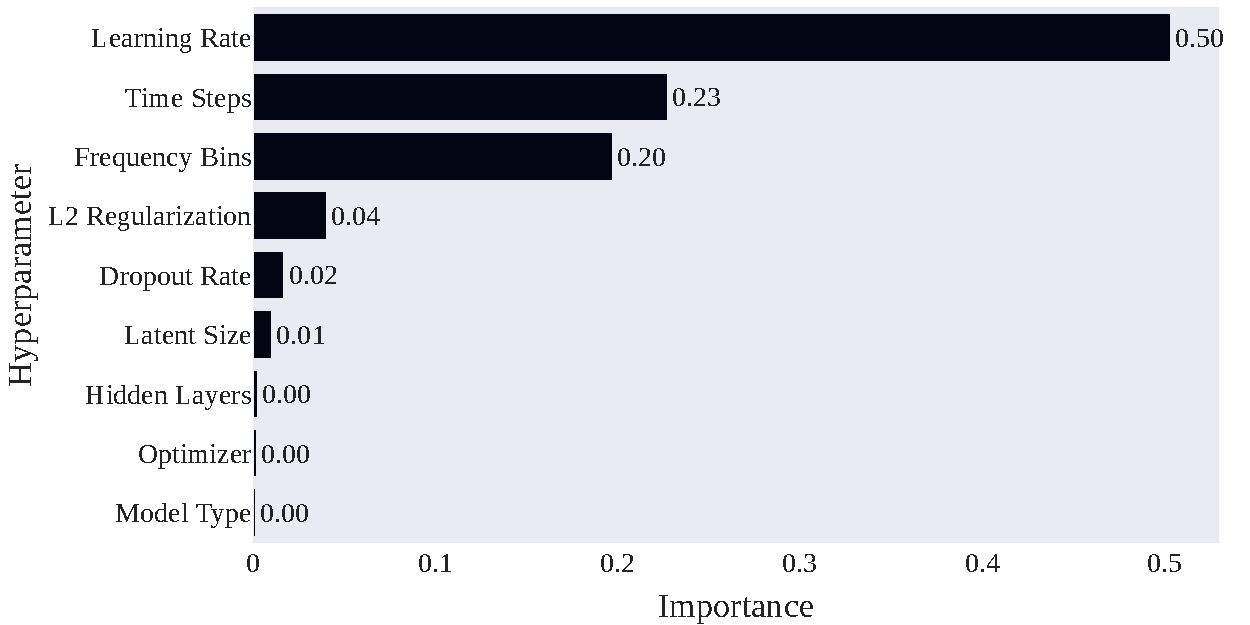
\includegraphics[width=14cm,height=7cm]{images/chapter_3/ParameterImportances_final.pdf}
\caption{The parameters' estimated importance in determining the outcome of trials. Specifications of the spectrogram seem to affect the outcome more so than the model's configuration. We attribute the contrast between the results here and those in Figure~\ref{fig:slicegraph} to the irregular rate of sampling from the hyper-parameter space.}
\label{chap3:param_importance}
\end{figure}

We depict the correlation of parameter values with trial results in Figures~\ref{fig:slicegraph}. We extract a more concrete measurement of hyper-parameter influence using the fANOVA importance evaluator~\cite{hutter2014efficient}. We limit this analysis to 500 trials with 20 epochs. The results of this estimation are depicted in Figure~\ref{chap3:param_importance}. Contrasting the results of the fANOVA evaluator with Figure~\ref{fig:slicegraph}, we notice several issues. Notably, the importance of 0 is attributed to \enquote{Model Type} and \enquote{Optimizer} parameters, despite a visible difference depicted in the slice-graph (Figure~\ref{fig:slicegraph}). This may be due to the imbalanced sampling of the hyper-parameter space, prompted by our greedy search in place of random sampling. Another possible cause is the \enquote{averaging} of loss results regardless of variance: For example, Figure~\ref{fig:slicegraph} depicts CNN models as having the best and worst results while FC models are reliably average; making the fANOVA's 0 importance attribution logical, but not optimal when we are strictly looking for the best models. 


% \subsection{Exploring Recursive Recreations}
% To gain some insight into the embedding mechanism, we create a  feedback loop where a decoded spectrograms are fed through the network again.
% We recursively run the autoencoder on new sounds and display the results in Figure~\ref{fig:recreations}. The results are displayed for 1, 2, 10 and 100 recursions. Spectrograms belonging to percussive groups retain their unique characteristics for many iterations, while details in most synthetic noise spectrograms are quickly dissipated. A major point of concern here is that recursively recreated synthetic noise spectrograms tend to take on drum characteristics. This is possibly prompted by our encoder only having been exposed to drums sounds prior.  Yet it is possible that the \enquote{confusion} demonstrated by the encoder after the initial reconstruction leads to embedding of familiar sounds being distinguishable from those unseen. 
% \begin{figure}[h!]
% \centering
% \textbf{Recursive Recreation of Drums and Synthetic Noise}\par\medskip
% \makebox[\linewidth][c]{%
% \begin{subfigure}[b]{.6\textwidth}
% \centering
% 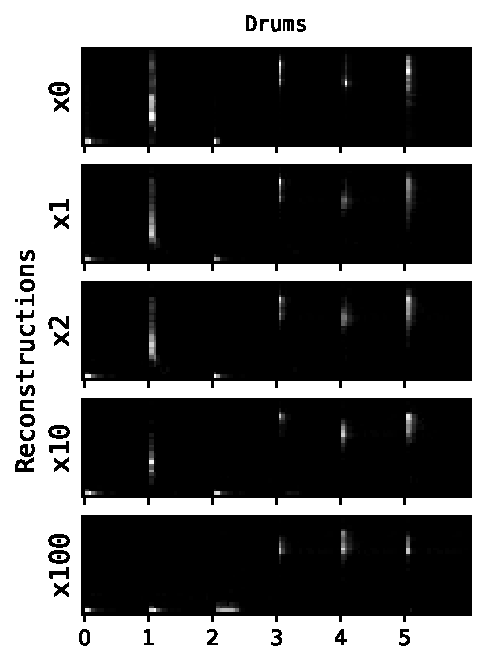
\includegraphics[width=.95\textwidth]{images/chapter_3/Drums_reacreation.pdf}
% % \caption{a test subfigure}
% \end{subfigure}%
% \begin{subfigure}[b]{.6\textwidth}
% \centering
% 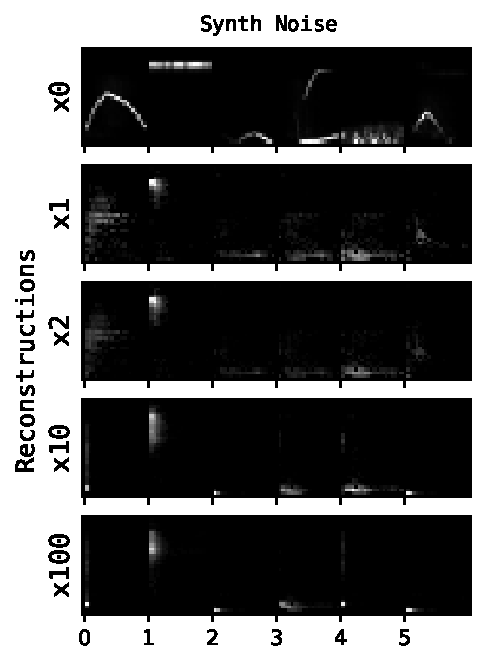
\includegraphics[width=.95\textwidth]{images/chapter_3/Synth Noise_reacreation.pdf}
% % \caption{a test subfigure}
% \end{subfigure}%
% }\\
% \caption{We concatenate 6 spectrograms for drum and synthetic noise groups. We recursively encode and decode these spectrograms and display the results. The first row depicts the unaltered spectrograms. We display the results after 1, 2, 10 and 100 recursive recreations. We see that drum spectrograms retain their original form better than synthetic noise.}
% \label{fig:recreations}
% \end{figure}




\subsection{Visualizing The Encodings}
\label{fig:embedding_FE}
\begin{table}[htbp!]
\centering
\begin{tabular}{|p{6cm}|p{6cm}|}
\hline
Hyper-Param. & Value  \\ \hline
Model Type      &  CNN  \\ \hline
Optimizer       & Adam  \\ \hline
Hidden Layers   & 1  \\\hline
Learning Rate   &  0.001145\\ \hline
Frequency Bins & 30 \\ \hline
Time Steps & 20 \\ \hline
Latent Size & 64 \\ \hline
Regularization & 3.25^{-6}\\ \hline
Dropout Rate & 0.5 \\ \hline
\end{tabular}
\caption{Top performing hyper-parameter set}
\label{table:best_params}
\end{table}
\begin{figure}[h!]
\centering
\textbf{2 Dimensional Projection of Latent Variables}\par\medskip
 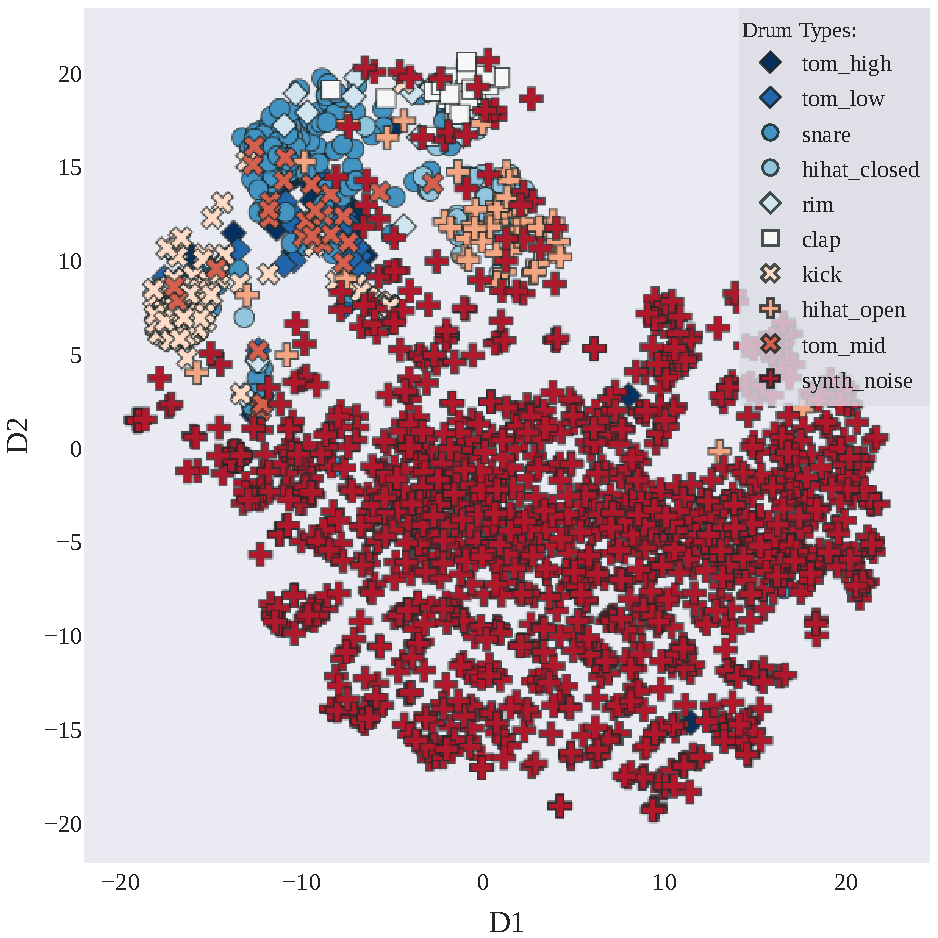
\includegraphics[width=0.90\linewidth]{images/chapter_3/t-SNE_2d.pdf}
\caption{Projection of an embedding model's low dimensional encoding on to a 2D plane. We implemented interactions for these graphs for manual inspection of samples.}
\label{fig:2d_tsne}
\end{figure}

\begin{figure}[htbp!]
\centering
\textbf{3D t-SNE Projection}\par\medskip
\mbox{\subfloat[]{\label{subfig:1} \fbox{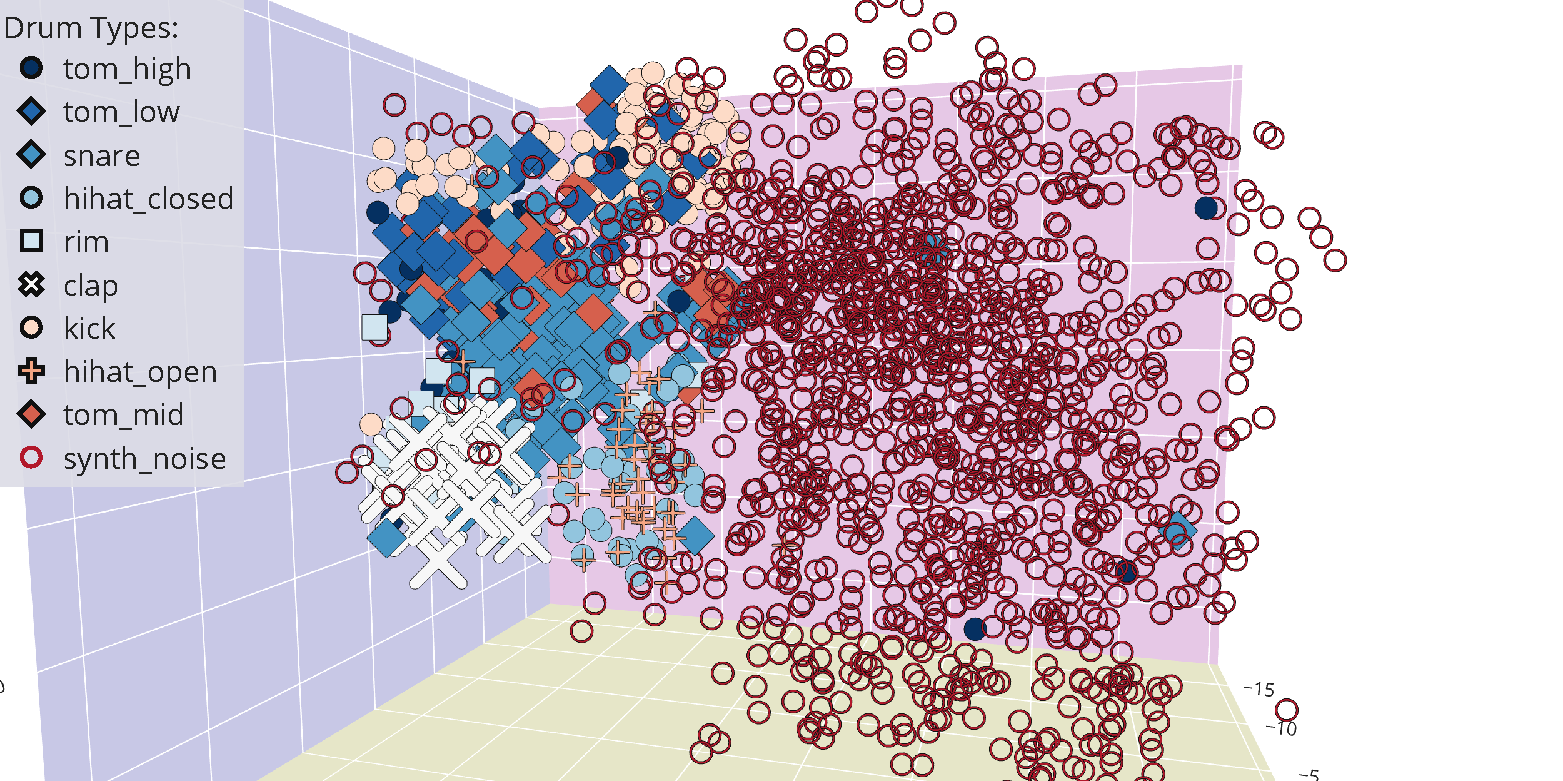
\includegraphics[width=14cm,height=6.8cm]{images/chapter_3/3d_t-SNE_symdrum_type_cam0.pdf}}}}

\mbox{\subfloat[]{\label{subfig:2} \fbox{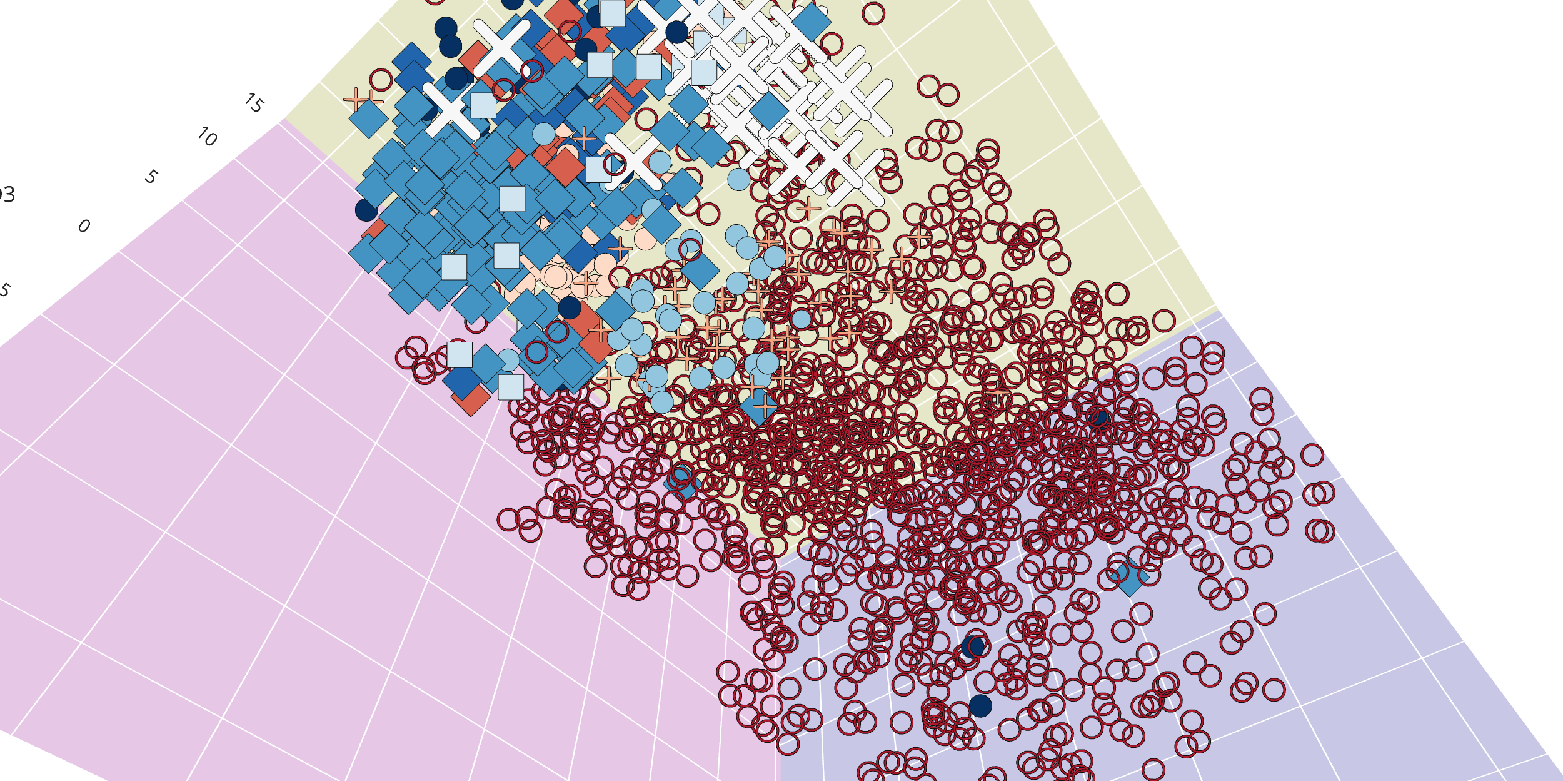
\includegraphics[width=14cm,height=6.8cm]{images/chapter_3/3d_t-SNE_symdrum_type_cam3.pdf}}}}

\fbox{\mbox{\subfloat[]{\label{subfig:2} 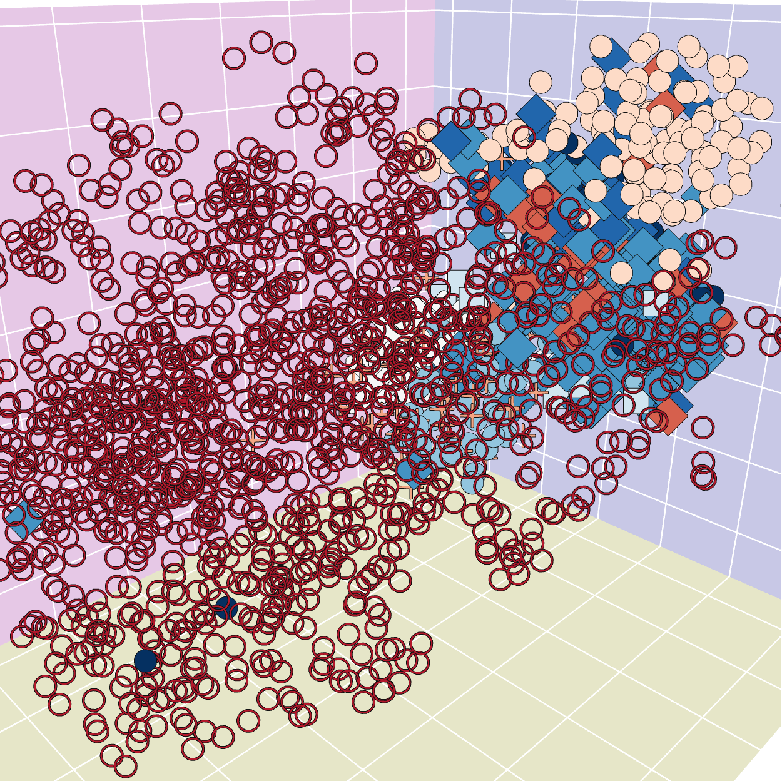
\includegraphics[width=5cm,height=5cm]{images/chapter_3/3d_t-SNE_symdrum_type_cam1.pdf}}}
\mbox{\subfloat[]{\label{subfig:2} 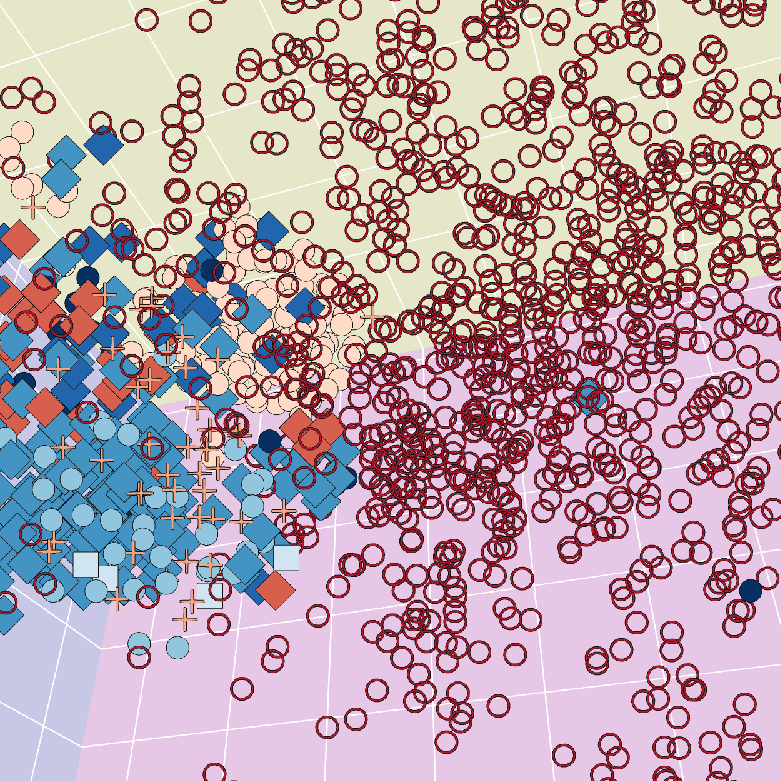
\includegraphics[width=5cm,height=5cm]{images/chapter_3/3d_t-SNE_symdrum_type_cam2.pdf}}}}
\caption{Our feature projections and interactive graphs can also be done in 3D}
\label{fig:3d_tsne}
\end{figure}

To better understand the delineation potential of the encoded features,  we trained an autoencoder with our top performing hyper-parameter set, shown in Table~\ref{table:best_params}. We used 80\% of MixedDB to train the model for 200 epochs. Using this model, we encoded the remaining 20\% and approximately 1000 randomly selected sounds from NoiseDB into 64 dimensions. These 64-dimensions were then projected onto a 2 or 3-dimensional plane using t-SNE. 

In the upcoming Section~\ref{sec:decisions}, we will thoroughly discuss the expectations of an effective virtual ear. In summary, if the embeddings are useful in helping the virtual ear with separation of drums from not-drums as well as categorization of drum types, we expect the projection of drum sounds to be clustered together, with the majority of the synthetic noise sounds appearing away from these clusters. Our projections confirm that this is the case. We are most interested in synthetic noise sounds which appear within or near these clusters. Do these synthetic noise sounds have drum like characteristics?\\ 

To test this, we implemented interactive graphs identical to those depicted in Figure~\ref{fig:2d_tsne} and~\ref{fig:3d_tsne}. These graphs allow for interactions such as playing the samples (by hovering the cursor on-top) and movement of the scene camera for a closer look at clusters.  Manual inspection reveals a noticeable, positive correlation between distance and similarity of a synthetic sound to a drum cluster. Divergences from the envelope features expected from drums are a common point of failure. A noticeable case was a synthetic noise resembling a \emph{reverse} kick drum within the kick cluster. While encouraging, we hypothesize that more specialized forms of encoding or addition of other features are needed for reducing the frequency of errors and strengthening this correlation.
\subsection{What To Do With Extracted Features}
\label{sec:howto_use_features}
So far, we discussed two methods of feature extraction for audio. The FFT features can represent various aspects of sound which may be helpful to a virtual ear. Using autoencoders, FFT features can be further condensed into small embedded spaces. These embedded spaces are harder to understand and explain, but the 2-dimensional projections shown in Figure~\ref{fig:2d_tsne}  indicate that they contain vital information about the different drum and non-drum sound types in our databases. 

The features discussed here can be used to train classifiers which can separate desirable from undesirable sounds. Section~\ref{TPE_models} covers the implementation of classifiers which directly use the FFT features and Section~\ref{chap3:mixed_ear_models} covers the use of embeddings to train virtual ear models. 
\section{Ear Decisions}
\label{sec:decisions}
 Having considered the caveats and requirements, once a sound is generated and passed onto the ear, we expect the virtual ear to make decisions in response to two important questions: 
\emph{
\begin{quote}
\text{Decision.1 Could the sound be used as a drum?}\label{Decision.1}
\\
\text{Decision.2 If it does sound like a drum, what type of drum should it be?}\label{Decision.2}
\end{quote}
    }
\decfirst~requires knowledge of what drums \textbf{do not} sound like, or knowledge of an infinitely large set, which cannot be fully represented via examples. An important consideration is that the source of sounds used for training the model (organic drum sounds) will be fundamentally different from the source of unlabeled sounds we wish to categorize (noise from a synthesizer). This issue is reflective of the open set recognition (OSR) problem~\cite{geng2020recent,mundt2019open}. Figure~\ref{fig:ven_data} highlights a number of caveats with our training approach. If the sound is deemed percussive, the virtual ear makes \decsecond~by finding the best drum category for the sound. The number of categories available is dependent on the database of drums used for training. 
% To maximize the transference of knowledge gained from training the classifiers to evaluation of programs, we need to extract concise feature sets that capture fundamental characteristics of the data points.

The goal is to create a pipeline of sound generation where the synthesizer is used for the rapid generation of sounds and the virtual ear is used for the acceptance of inputs which satisfy some fundamental characteristics of percussive instruments. The representation of sounds is critical in allowing the acceptance of novel sounds as part of the drum group despite their anomalies. In Section~\ref{chap:represent_sound}, we discussed 2 different approaches to feature extraction. This leads to two different implementation of a virtual ear: \emph{two phased ears} (TPEs) and \emph{mixed ear models} (MEMs). TPEs are a combination different models for each of \decfirst~and \decsecond. The features utilized by these models are manually defined. MEMs use a highly compressed, automatically encoded representation of sound to give simultaneous answers to both questions.


\subsection{Two Phased Ears}
\label{TPE_models}
\begin{figure}[t!]
    \begin{center}
    \textbf{TPE Design}
    \makebox[\textwidth]{
    \fbox{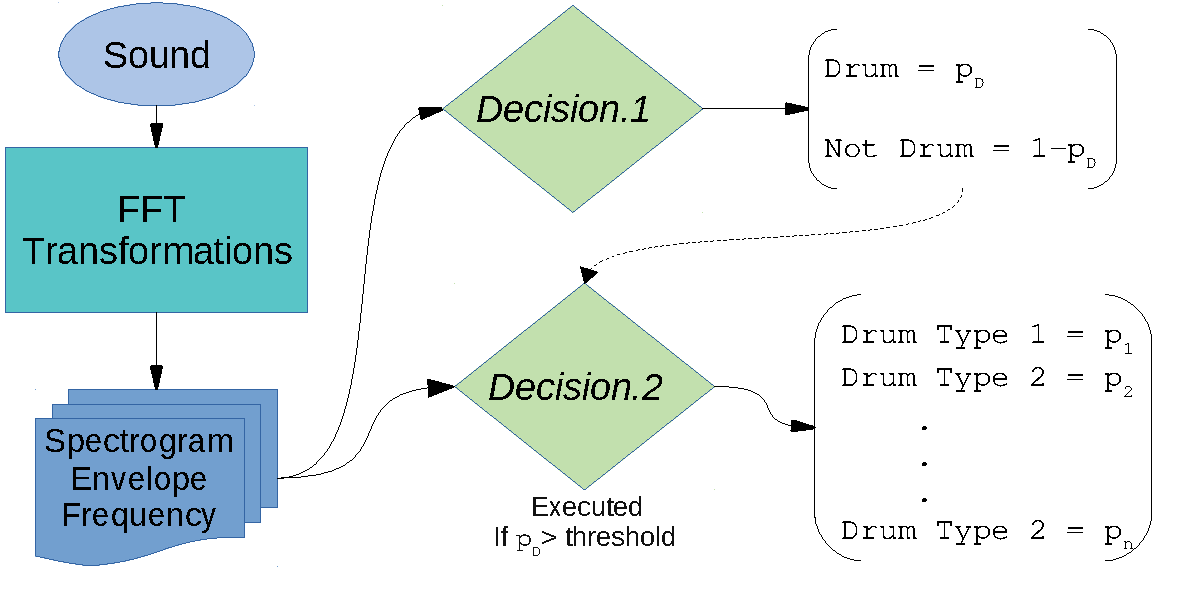
\includegraphics[width=1.1\linewidth]{images/chapter_4/TPE_ear.pdf}}}
    \end{center}
    \caption{TPE's receive a sound and make decisions sequentially.}
\label{fig:TPE_design}
\end{figure}

Using the features and transformation described in the previous section as input, we trained several neural network models with the pytorch library. The tasks at hand with regards to \decfirst~is to separate drums from not-drums (DrumVsNotDrum, or DVN). In \decsecond~the aim is to categorize the type of drums and percussion (DrumVsDrum, or DVD). 

 Multiple neural network architectures using different subsets of the FFT features to specialize in \decfirst~or \decsecond~are combined to make decisions sequentially. For \decfirst, all drums in RadarDB and FreeDB and 6000 examples of virtual synthesizer noise are used. For \decsecond, we combined the two databases and merge toms into kicks and rims/shakers into \enquote{other}. 80\% of this dataset were used for training, and the remaining 20\% of sounds for testing. 98\% accuracy in \decfirst~and 82\% accuracy in~\decsecond~were achieved with the best models. The loss function and optimizer are Categorical Cross-Entropy and Adam respectively. Training continued until no reduction in loss and accuracy is observed for 10 epochs. These accuracy numbers are weak as we did not account for category sizes or cross validate.  


\subsubsection{DVN Models}
\textbf{FC-DVN}: Fully connected network trained on Envelope features, reaching 97\% accuracy on the test data for~\decfirst. 
\begin{center}
\vbox{
    \begin{lstlisting}[caption=Sequential Layers for FC-DVN]
            Layer                       Details
            ========================================================
            Linear                      in_features=400 
                                        out_features=20 
                                        bias=True
            PReLU                       
            Linear                      in_features=20
                                        out_features=10 
                                        bias=True
            PReLU
            Linear                      in_features=10
                                        out_features=4
                                        bias=True
            PReLU
            Linear                      in_features=4
                                        out_features=2
                                        bias=True
            Softmax                     DVN probabilities
                        
        \end{lstlisting}}
\end{center}
\textbf{CNNLSTM-DVN}: A combination of CNN and LSTM models, where the CNN model extracts higher level features that are fed temporally to an LSTM cell. This model is trained on spectrum data and reaches 98\% accuracy on the test set. 
\begin{center}
\vbox{
    \begin{lstlisting}[caption=Sequential Layers for CNNLSTM-DVN]
            Layer                       Details
            ========================================================
            Conv2d                  kernel size = (7, 3)
                                    stride = (1, 1)
                                    padding = (3, 1)
            ReLU
            Dropout                 probability = 0.5
            LSTMCell                hidden size = 800
                                    input size = @($\mathcal{F}$)@
            Linear                  in_features = @($\mathcal{F}$)@
                                    out_features = 2
                                    bias=True
            Softmax                 DVN probabilities
\end{lstlisting}}
\end{center}

\subsubsection{DVD Models}
\textbf{E+F-DVD}: A fully connected model trained on a concatenation of envelope and frequency features. Reaching 80\% accuracy for 6-way drum categorization in Phase 2. 
\begin{center}
\vbox{
    \begin{lstlisting}[caption=Sequential Layers for E+F-DVD]
            Layer                       Details
            ========================================================
            Linear                      in_features = 10+50 
                                        out_features = 30
                                        bias = True
            PReLU                       
            Linear                      in_features = 30
                                        out_features = 10
                                        bias = True
            PReLU                       
            Linear                      in_features = 10
                                        out_features = 10
                                        bias = True
            PReLU     
            Linear                      in_features = 10
                                        out_features = @($\mathcal{C}$)@
                                        bias = True
            Softmax                     drum type probabilities
        \end{lstlisting}}
\end{center}

\textbf{CNN-DVD}: A CNN model trained on Spectrum features. Reaching 82\% accuracy in a 6-way drum categorization in Phase 2.  
%  {\color{red}double check architecture}
\begin{center}
\vbox{
    \begin{lstlisting}[caption=Sequential Layers for CNNLSTM-DVD]
            Layer                       Details
            ========================================================
            Conv2d                  kernel size = (7, 3)
                                    stride = (1, 1)
                                    padding = (3, 1)
            ReLU
            Dropout                 probability = 0.5
            LSTMCell                hidden size = 800
                                    input size = @($\mathcal{F}$)@
            Linear                  in_features = @($\mathcal{F}$)@
                                    out_features = 2
                                    bias=True
            Softmax                 DVD probabilities
\end{lstlisting}}
\end{center}

\textbf{FC-DVD}: Fully connected 3 layer neural net with 78\% accuracy for 6-way drum categorization in Phase 2. 
\begin{center}
\vbox{
    \begin{lstlisting}[caption=Sequential Layers for FC-DVD]]
            Layer                       Details
            ========================================================
            Linear                      in_features=400
                                        out_features=20 
                                        bias=True
            PReLU                       
            Linear                      in_features=20
                                        out_features=10 
                                        bias=True
            PReLU
            Linear                      in_features=10
                                        out_features=4
                                        bias=True
            PReLU
            Linear                      in_features=4
                                        out_features=@($\mathcal{C}$)@
                                        bias=True
            Softmax                     drum type probabilities
                        
        \end{lstlisting}}
\end{center}



\subsection{Mixed Ear Models}
\label{chap3:mixed_ear_models}
\begin{figure}[t!]
    \begin{center}
    \textbf{MEM Design}
    \makebox[\textwidth]{
    \fbox{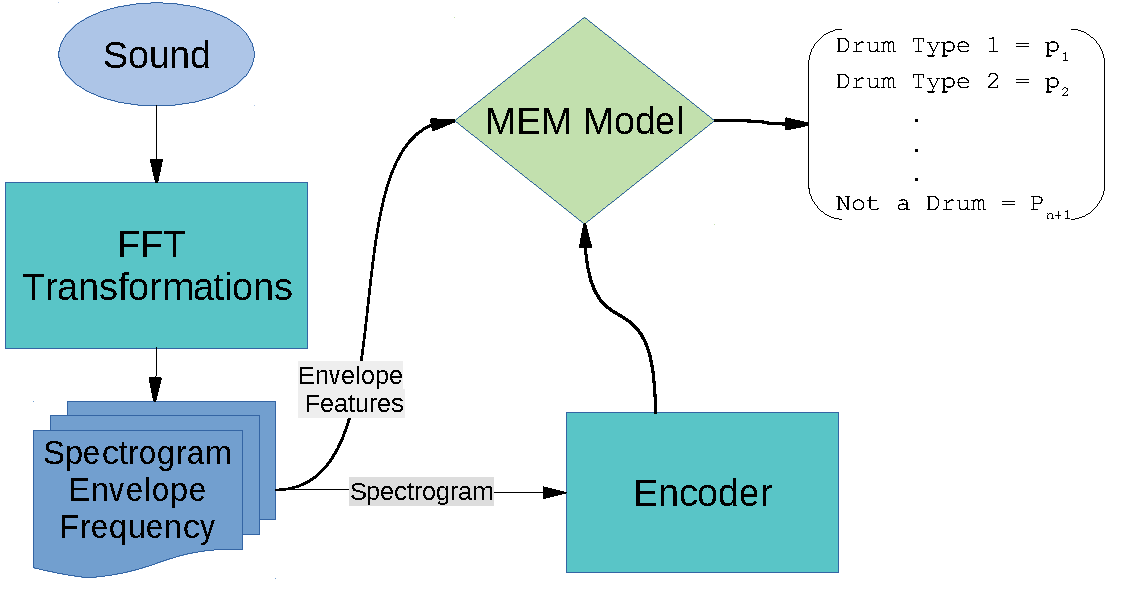
\includegraphics[width=1.1\linewidth]{images/MEM_ear.pdf}}}
    \end{center}
    \caption{MEMs use both FFT features and embedding features to make both decisions simultaneously. }
\label{fig:TPE_design}
\end{figure}

Unlike TPEs which make their decisions in two steps, mixed ear models (MEMs) simultaneously categorize a new sound's drum type or put it in the \enquote{synthetic noise} category. We call this task drum vs drum vs not-drum, or \enquote{DvDvN}.

Manual t-SNE inspections discussed in Section~\ref{fig:embedding_FE} highlighted a disregard for envelope shapes as a major source of failure. Because of this, the feature set used to train MEMs contains envelope and embedded features. The performance of the models before and after the addition of envelope features (a vector of size 10) to the feature space is shown in Figures~\ref{fig:f1_allg_box} and~\ref{fig:f1_dvn_box}.

The autoencoder model trained on MixedDB is used as an embedding feature extractor. RadarDB, FreeDB and NoiseDB are combined for training/test data. To prevent class overlaps as much as possible, only claps, hats, kicks, snares and synthetic noise groups are used for measuring model effectiveness. Samples longer than 1 second are excluded in order to reduce potentially mislabeled data. This combined dataset was described in Section~\ref{db:memDB}


\subsubsection{Model Selection}
Using embeddings and envelope features to represent audio, five classification models were trained for the task of categorizing the five different sound groups. We did not use neural networks for classification as traditional classification models have been shown to match, if not exceed deep-learning models with less training time, given that the feature set is a simplified representation extracted using neural networks~\cite{notley2018examining}.

 We arbitrarily select 5 traditional classification models from the scikit-learn library (version 23)~\cite{pedregosa2011scikit}. The 5 classification models used and their hyperparameters are presented in Table~\ref{table:mem_model_selection}, and any unmentioned hyperparameters are set to the library's defaults. To compare the models, we conducted a 10-fold cross validation and plot the F-scores in Figure~\ref{fig:f1_allg_box}. Each of the 10 F-scores reported is the average F-score when classifying individual drum groups. Class weights were used where possible to mitigate the effects of an imbalanced dataset~\cite{provost2000machine,chawla2004special}. When utilized, the weight for each class $c$ is calculated as:

\begin{subequations}
    \begin{align*}
    c_{weight} = 1-\dfrac{\text{Number of samples in group $c$} }{\text{Total number of samples}}
    \end{align*}
\end{subequations}

\begin{table}[t]
    \centering \hspace*{-0.8cm}
    \begin{threeparttable}
    \begin{tabular}[width=0.95\paperwidth]{|l|l|l|}
    \hline
    Model name & Modified Parameters\tnote{\dag}  & Used Weights? \tnote{\ddag} \\\hline
     Support Vector Classifier (SVC) &  Gamma:0.001, C:100, kernel:rbf & Yes\\
     LinearSVC & C:10 & Yes\\
     K Nearest Neighbors & Number of Neighbors:31 &  No \\
     Random Forest Classifier & Number of Estimators:500 & Yes \\
     Extra Trees Classifier & Number Estimators:1100 & Yes\\
     \hline
    \end{tabular}
    \caption{Models implemented for comparison using envelope and embedded features. }
    \begin{tablenotes}
    \item[\dag] Parameters not mentioned have neither been tuned nor changed from scikit-learn's default values (as of version 0.23)
    \item[\ddag] Class weights are used unless not applicable to classifier.
    \end{tablenotes}
    \label{table:mem_model_selection}
    \end{threeparttable}
\end{table}

\begin{figure}[htbp!]
    \begin{center}
    \textbf{Cross Validation F-Scores For All Sound Groups}\par\medskip
    \makebox[\textwidth]{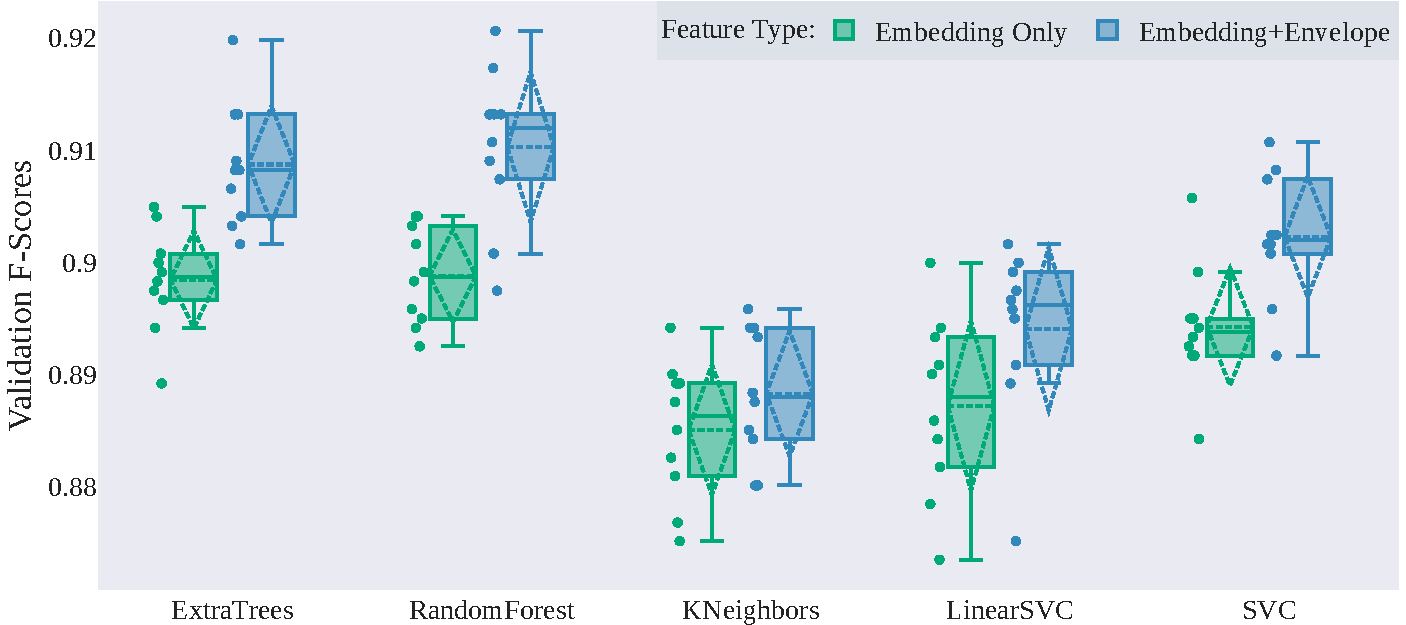
\includegraphics[width=0.8\paperwidth]{images/chapter_3/mme_comparisons_mme.pdf}}
    \caption{Boxplots visualizing the F-Score results for each cross-validation. The individual scores, means, medians, standard-deviation and outliers are depicted. The differences are noticeable, yet means lie within the \%88-92 range. Envelope features improve classification accuracy for all models. }
    \label{fig:f1_allg_box}
    \end{center}
\end{figure}

To see how these models perform on the binary DvN task (i.e \decfirst), the performance of the models is measured in the same manner after all drums are grouped together. The results of these tests are shown in Figures~\ref{fig:f1_allg_box} and~\ref{fig:f1_dvn_box}. Considering the performance of these models, we selected the extra-trees model as the most promising model for the virtual ear. Extra-trees is an ensemble-model which uses the results of multiple random forests trained on different feature subsets~\cite{geurts2006extremely,pedregosa2011scikit}.

\begin{figure}[htbp]   
    \begin{center}
        \textbf{Cross Validation F-Scores For Drum Vs Not-Drum}
    \makebox[\textwidth]{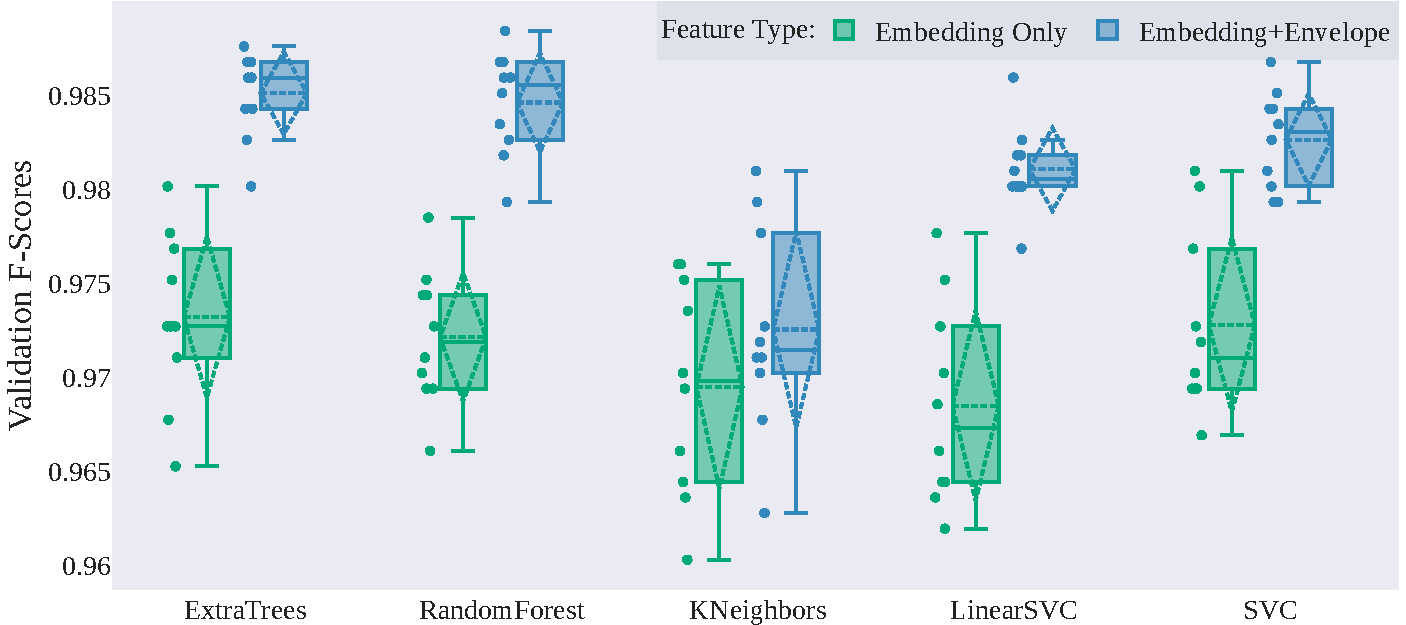
\includegraphics[width=0.8\paperwidth]{images/chapter_3/mme_comparisons_dvn.pdf}}
    \caption{F-Score results for each cross-validation. Models perform better as there are less categorization groups. Envelope features increase accuracy for all models. Random Forest and Extra Trees remain the top two models. }
    \label{fig:f1_dvn_box}
    \end{center}
\end{figure}


\begin{figure}[htbp]
\begin{center}
    \textbf{ Classification Report for DvDvN and DvN  }\par\medskip
    \makebox[\textwidth]{
    \subfloat[Precision, recall, F1-Score, and number of supporting examples]{ 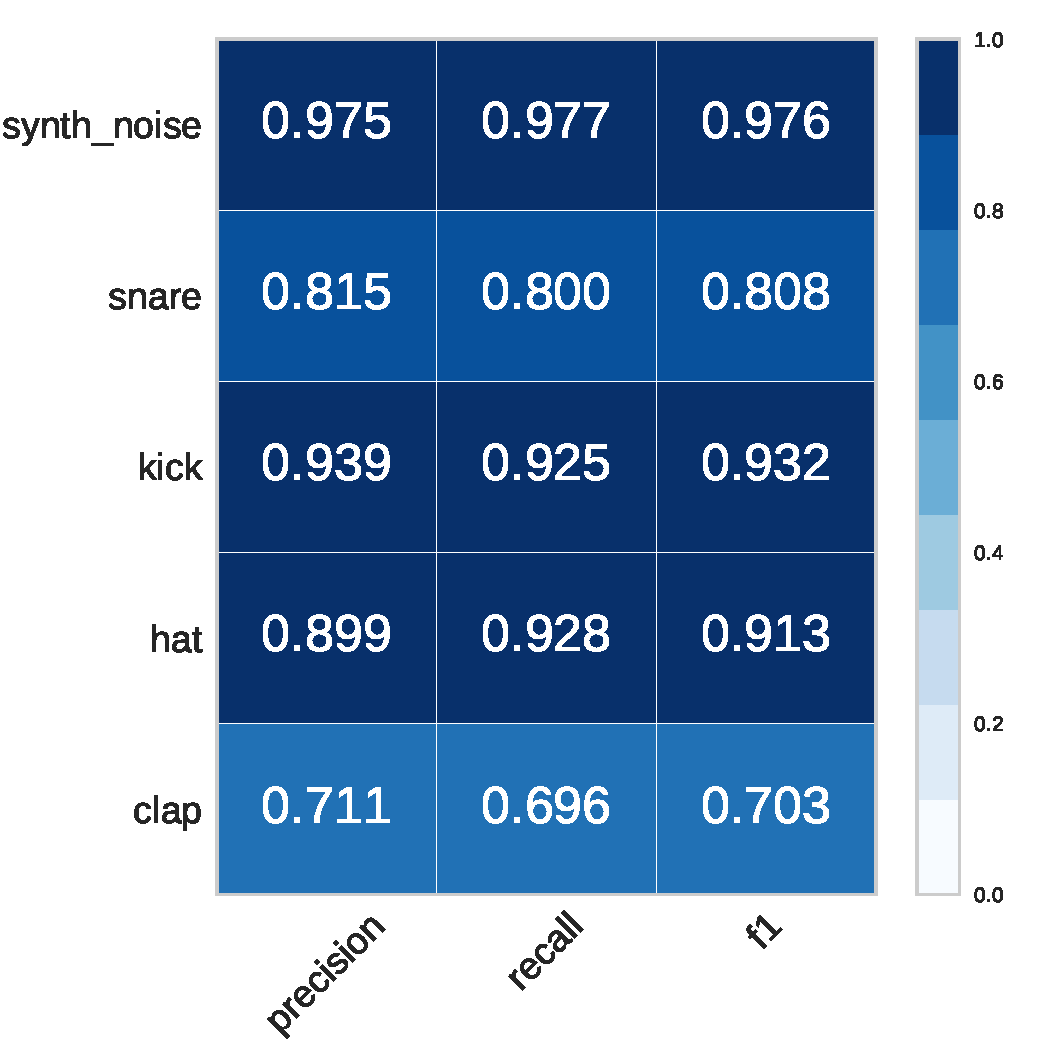
\includegraphics[width=9cm,height=9cm]{images/chapter_3/f1_mme.pdf}
    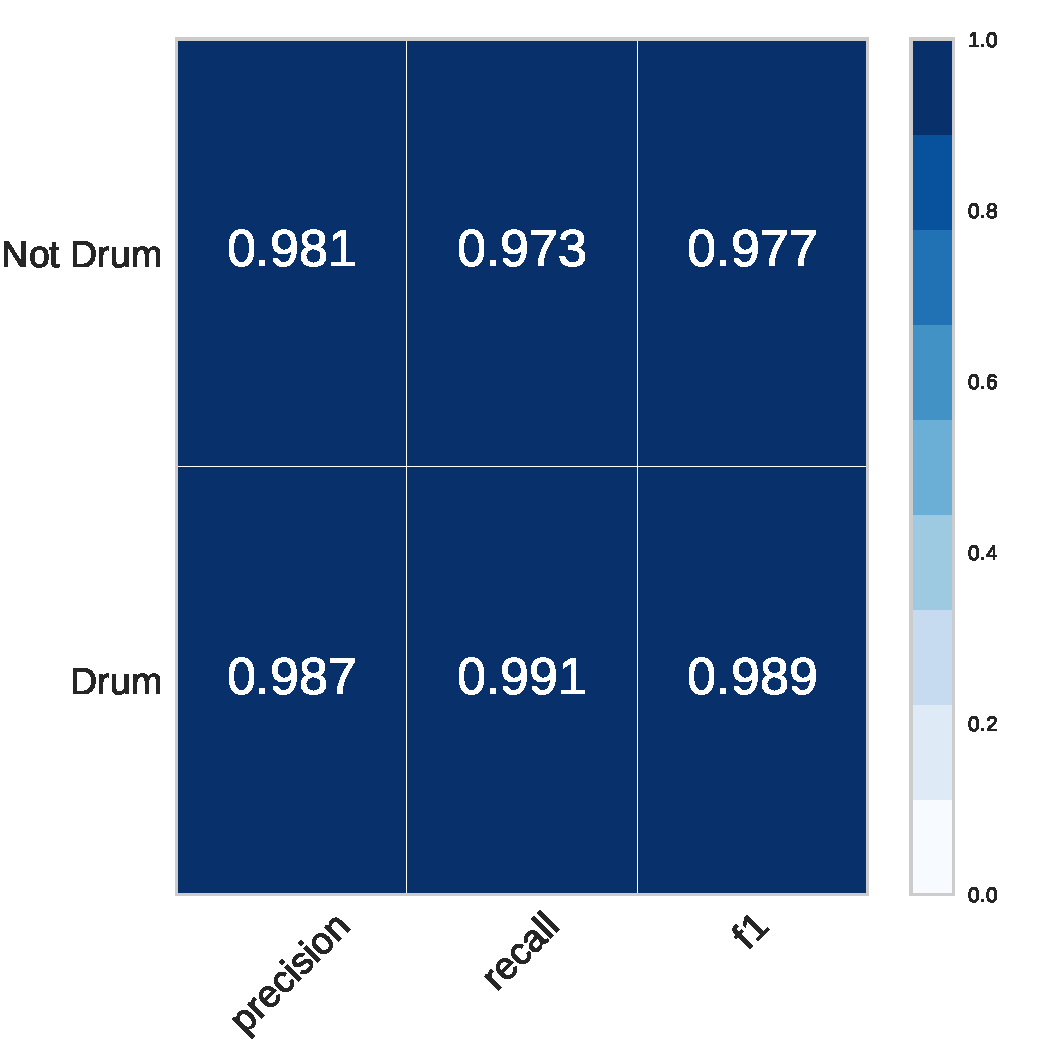
\includegraphics[width=9cm,height=9cm]{images/chapter_3/f1_dvn.pdf}
    }
    
    }
\label{fig:conf_f1_dvd}
\end{center}

\begin{center}
    \makebox[\textwidth]{
    \subfloat[Confusion matrices]{ 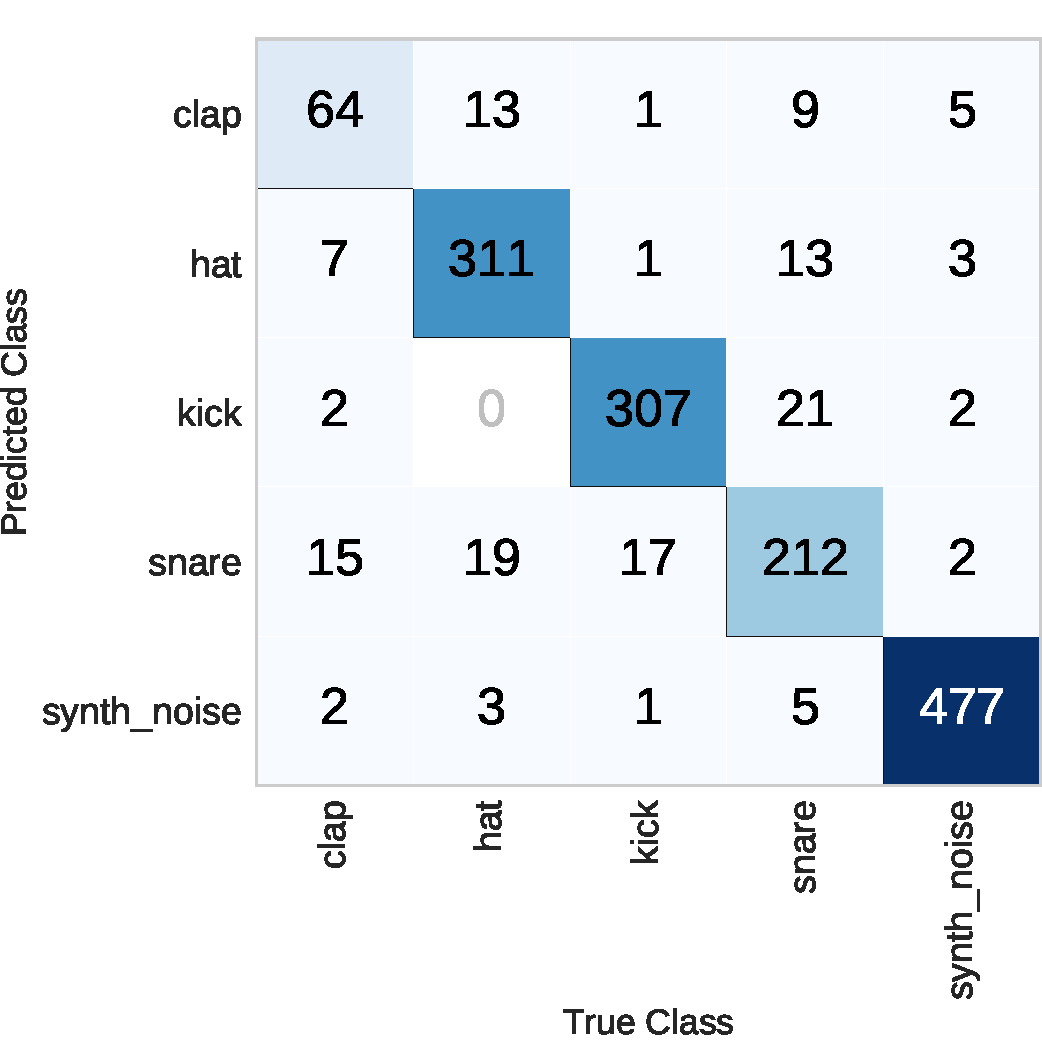
\includegraphics[width=9cm,height=9cm]{images/chapter_3/conf_mme.pdf}
    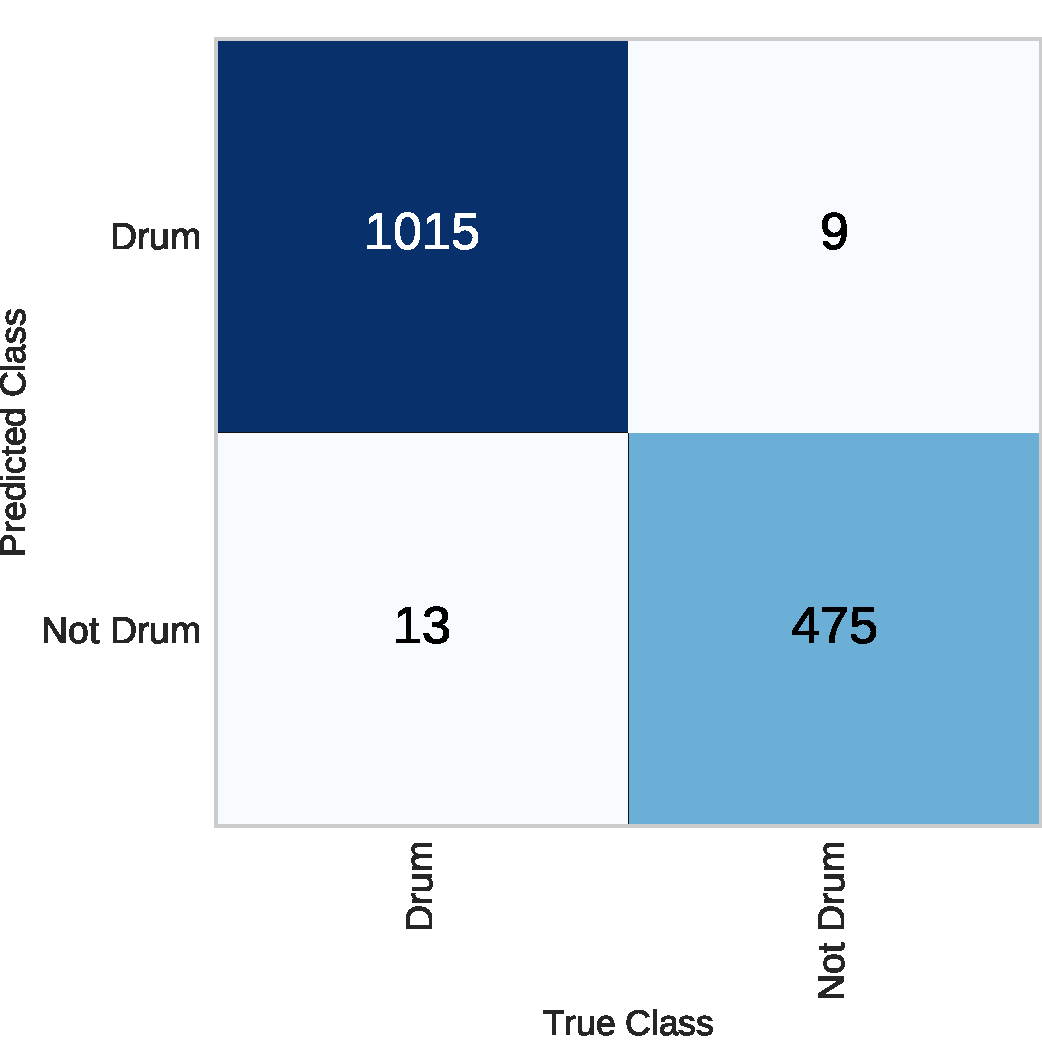
\includegraphics[width=9cm,height=9cm]{images/chapter_3/conf_dvn.pdf}
    }}
\end{center}


\caption{F-Scores and confusion matrix of ExtraTrees model for both DvDvN and DvN categorization.}
\label{fig:conf_f1_dvn}
\end{figure}

To create the confusion matrices and the F-Scores shown in Figure~\ref{fig:conf_f1_dvn}, the extra-trees model was trained on 80\% of the database, and tested with the remaining 20\%. Based on these reports, having multiple options for drum categorization does not noticeably influence the models accuracy in \decfirst. The DvDvN model's slightly smaller false negative rate for synthetic noise (11 vs 13 false negatives) is countered by a slightly higher rate of categorizing drums as synthetic noise (12 vs 9). Going forward, the DvDvN implementation is used as it makes the DvN model redundant. The finalized MEM used in the subsequent chapters is created by combining the autoencoder model with the ExtraTrees DvDvN classifier. 

% the addition of envelope features had a positive effect on performance for all models, yet the RandomForest and ExtraTrees models clearly outperform the other classifiers in both tasks.

\section{How Will TPEs and MEMs Be Used?}
With the virtual synthesizer in place, we required a virtual ear: a tool capable of automatic separation of drums from non-drums and categorization of drum sounds.  We took two different approaches to implementing such a tool, which gave us two types of virtual ears: TPE Ears, which make the two decisions sequentially, and MEM ears which makes these decisions simultaneously. The distinguishing characteristic of TPEs and MEMs is the type of feature set that they use for learning. TPEs use envelope and spectrogram features derived using Fourier transformations, while MEMs use encoded spectrogram features, which is a much smaller set of features, yet achieve similar classification performance.  

 Based on results shown in this chapter, TPEs and MEMs appear to have high categorization accuracy in our testing data. But without manual hearing tests, we cannot know whether the synthesizer sounds that are deemed percussive by the virtual ears resemble organic drum sounds or simply have characteristics that the virtual ears were not familiar with, leading to mistakes. This is due to the infinite variety of sounds that are not percussive (i.e, the OSR problem), which makes such training tasks difficult. 
 
In the next chapter we first discuss how TPEs and MEMs are used to implement generative systems capable of outputting percussive sounds and how the outputs of these systems were manually tested in order to measure their success in creation of drum sounds. We also discuss how this success hinges on the virtual ear's ability in separation drums from non-drums as well as accurate categorization of drums. 

 
% With the models showing high accuracy on testing data, they are combined in order to make decisions sequentially. The final implementations are manually tested, and the results are discussed in the Chapter~\ref{surveys}. \decfirst~we only determine sounds as percussive if both FC-DVN and CNN-LSTM have categorized it as such with over 90\% confidence. For \decsecond, the agreement between human listeners and each drum-vs-drum is measured.

% For the majority of random generations, that is not the case, but if a randomly generated sound has passed this phase, the three categorizers assign their categorizations to this sound.  These categorizers have a moderate degree of agree-ability as seen in Section~\ref{surveys}, but often the decision is not unanimous.
% TPEs can be combined and weighted in various ways and the confidence thresholds can be modified in order to implement \enquote{virtual ears} with different properties. A glaring issue in the current implementation is the treatment of softmax outputs as a reasonable measure of a model's confidence. As a result, some models may have unwarranted higher confidence in their scores, skewing attempts at finding a consensus.  



% The fourth method of categorization, \enquote{averaged-cat}, is implemented by taking the sum of the softmax outputs of all three categorizers, using it to determine the category.




% \subsubsection{How TPEs Are Used}

% With the models showing high accuracy on testing data, they are combined in order to make decisions sequentially. The final implementations are manually tested, and the results are discussed in the Chapter~\ref{surveys}. \decfirst~we only determine sounds as percussive if both FC-DVN and CNN-LSTM have categorized it as such with over 90\% confidence. For \decsecond, the agreement between human listeners and each drum-vs-drum is measured.

% For the majority of random generations, that is not the case, but if a randomly generated sound has passed this phase, the three categorizers assign their categorizations to this sound.  These categorizers have a moderate degree of agree-ability as seen in Section~\ref{surveys}, but often the decision is not unanimous.


% \section{Is the Virtual Synthesizer Deterministic?}
% \label{section:synth_deterministic}
% It is crucial that rendering the audio from the same synthesizer program results in identical, or near identical sounds. Our synthesizer modules are capable of producing random waves, or \enquote{noise}. This type of sound will vary each time it is produced. Manual listening does not show sonic variation between multiple creation of the same set of parameters, but how does this affect the ear models?

% We create 50 parameter sets for stack sizes of 1 and evaluate each parameter set 10 times using the CNN-DVN model. This model outputs the probability of a sound belonging to the drum/percussion category (Discussed previously in Section~\ref{TPE_models}). Put simply, we are creating the sonic output given the same program multiple times and recording the predicted value from the model. We repeat this experiment for stack sizes of 2 and 8 and show the results in Figure~\ref{fig:synth_deterministic}. 

% \begin{figure}[htbp!]
% \begin{center}
%     \textbf{ Variation in Repeated Evaluations of Synthesizer Programs }\par\medskip
%     \makebox[\textwidth]{
%     \subfloat[1 Stack]{ 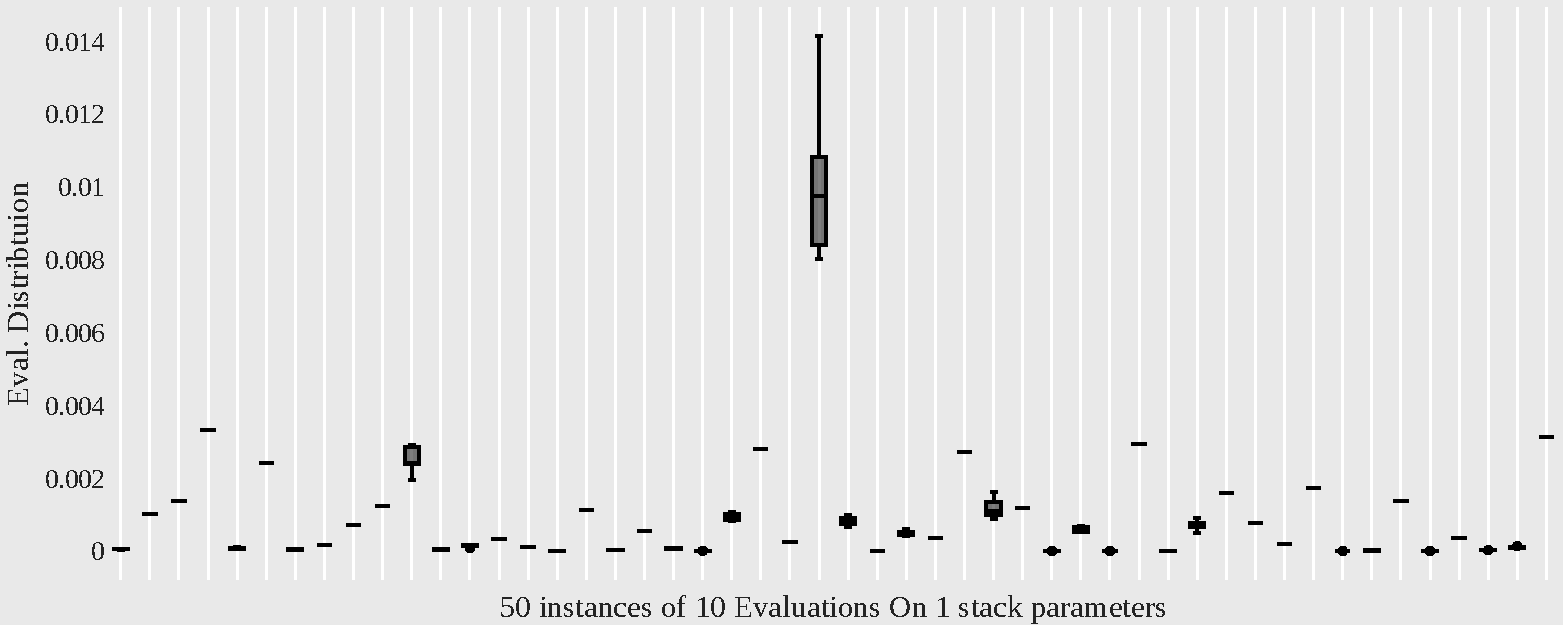
\includegraphics[width=17cm,height=5.67cm]{images/chapter_3/eval_stability_stacksize1.pdf}

%     }}

%     \makebox[\textwidth]{
%     \subfloat[2 Stacks]{ 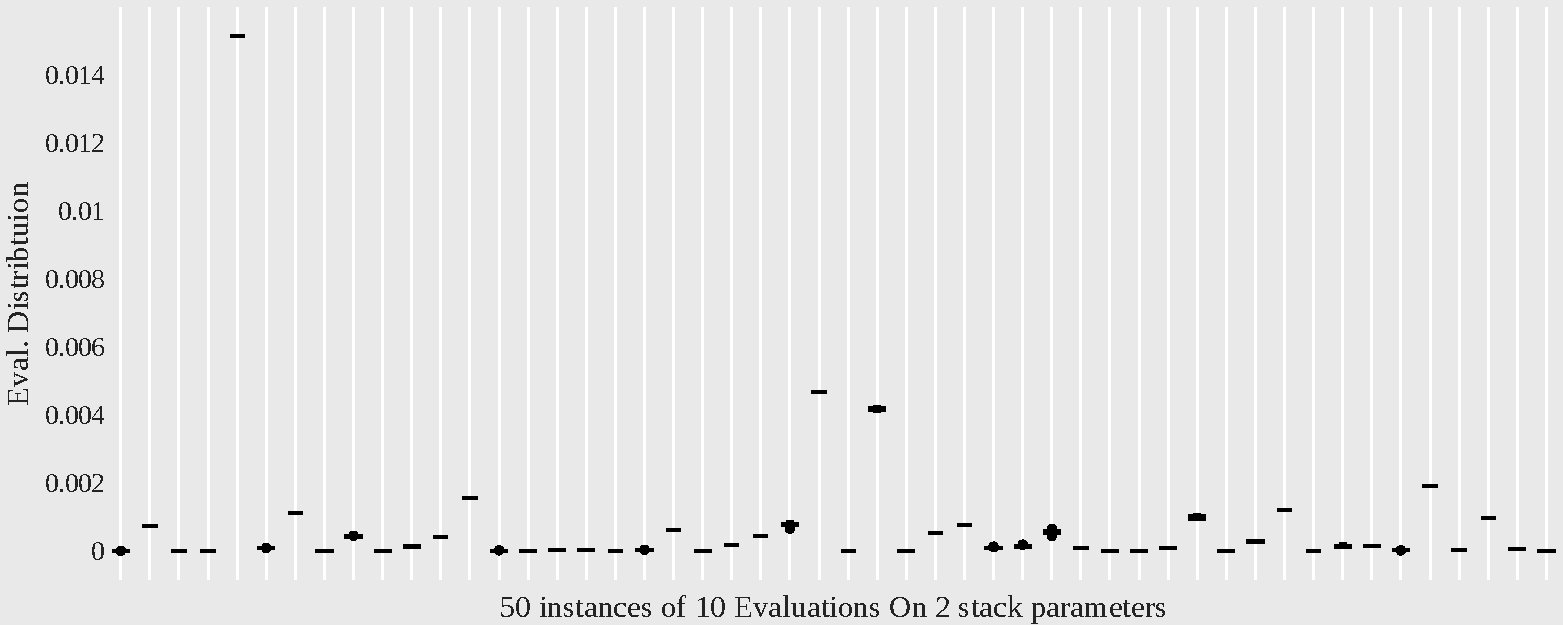
\includegraphics[width=17cm,height=5.67cm]{images/chapter_3/eval_stability_stacksize2.pdf}

%     }}
    
%     \makebox[\textwidth]{
%     \subfloat[8 Stacks]{ 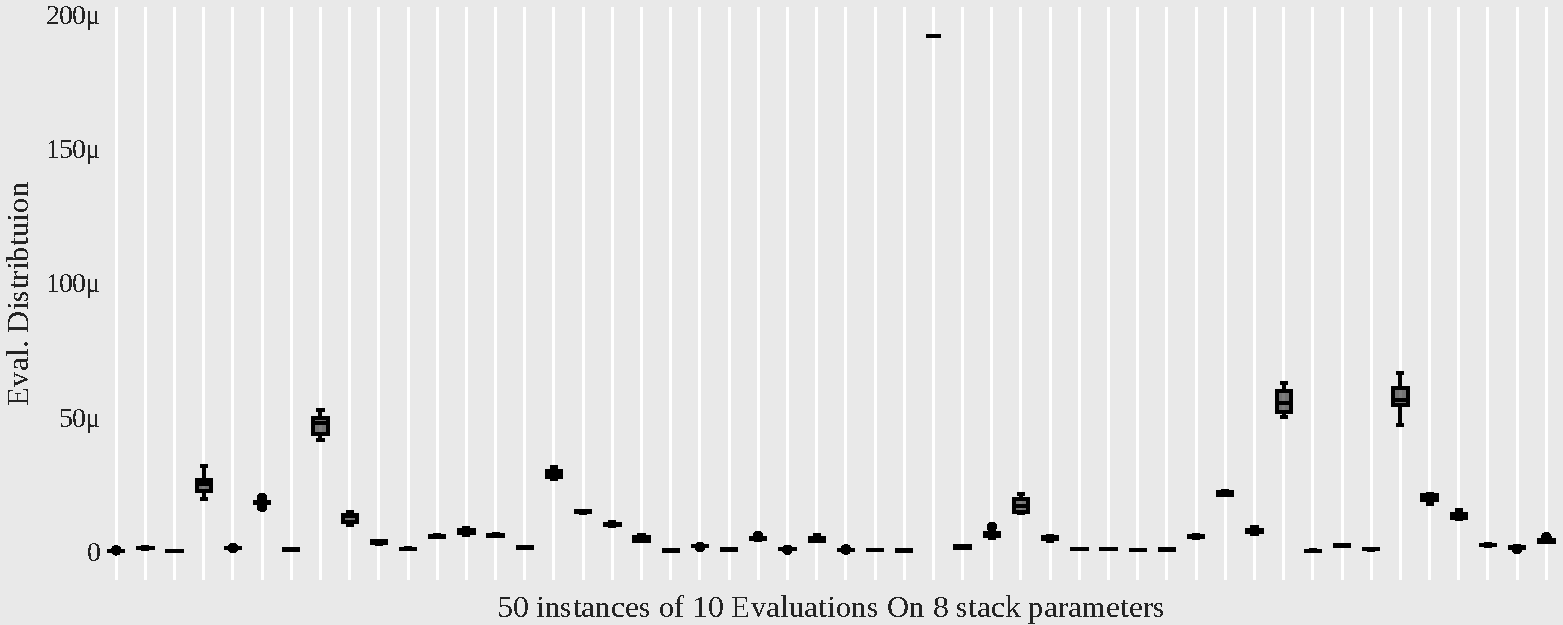
\includegraphics[width=17cm,height=5.67cm]{images/chapter_3/eval_stability_stacksize8.pdf}

%     }}
% \end{center}

% \caption{Repeated evaluation of signals from identical paramter-sets shows little variation in scores. Multiple renditions of the same parameter-set vary if the parameter-set calls for generation of 1 or more random wave-shapes..}
% \label{fig:synth_deterministic}
% \end{figure}



\end{document}